\chapter{Memory formation in Alzheimer's Disease}
\section{Introduction}

\section{Material and Methods}

\subsection{Animals and vectors}
All mice were housed in groups of 3--5, with a 12-hour light/dark cycle. Food and water are provided \textit{ad libitum} to all mice. Experiments were performed during the light phase of the circadian cycle. Mice were at least 8 weeks old at the beginning of all experiments. All experiments were conducted in accordance to the Hospital for Sick Children Animal Care and Use Committee.

\subsubsection{TgCRND8 mice}
TgCRND8 mice were developed at the Centre of Research for Neurodegenerative Diseases (CRND) and carry a human APP695 transgene with the Swedish (K670N-M671L) and Indiana (V717F) FAD mutations under the regulation of the Syrian hamster prion promoter \citep{chishti01}. Transgenic mice were maintained in a 129S6/SvEvTac background. TgCRND8 was then crossed with either \gls{wt} C57BL/6NTac or GP5.17. \Gls{tg} and \gls{wt} litter-mates of F1 generation were used in the experiments.


\subsubsection{GP5.17 mice}
GP5.17 mice transgenically express the fluorescence calcium indicator GCaMP6f under the Thy1 promoter \citep{dana14}. Offspring of TgCRND8 $\times$ GP5.17 positive of GCaMP6f and negative for \gls{app} were included in the \gls{wt} group. Double positive offspring were included in the \gls{tg} group.


\subsubsection{Viral vectors}
In the TgCRND8 mice, GCaMP6f expression is delivered through \gls{aav}. GCaMP6f expression is controlled by \gls{hsyn} promoter. AAV--DJ--syn--GCaMP6f virus was purchased from Stanford University Gene and Viral Vector Core and used undiluted. 

\subsubsection{\tglu peptide}
To deliver \glu construct (\texttt{YKEGYNVYG}) to target, we attached it to the protein transduction domain of the \gls{hiv} \textit{tat} gene (TAT peptide). The TAT peptide is able to transport across cell membrane and \gls{bbb} through a mechanism which is still unknown \todo{cite TAT}. The \tglu was synthesized from the sequence \texttt{YGRKKRRQRRRYKEGYNVYG}. It was injected in saline solution.


\subsection{Viral Infusion}

Each mouse received \gls{ip} injection of atropine (\SI{0.1}{\mg\per\kg}) and chlorohydrate (\SI{400}{\mg\per\kg}) before being secured on a stereotaxic frame. An incision was made on the scalp and the skin was pulled to the side to reveal the skull. Holes were drilled above \gls{la} on the skull for micropipette injection. Virus was loaded into a glass micropipette and gradually lowered to target coordinate. \SI{1.5}{\ul} of virus were injected on each side at a rate of \SI{0.12}{\ul\per\min}, aiming at \gls{la} (\gls{a/p} \SI{-1.4}{\mm}, \gls{m/l} $\pm$\SI{3.5}{\mm}, \gls{d/v} \SI{5.0}{\mm} from Bregma). The micropipette was left in the brain for an extra \SI{10}{\min} before slowly retracted. The incision was sutured and treated with antibiotics. Each mouse then received subcutaneous injection of analgesic (ketoprofen, \SI{5}{\mg\per\kg}) before returned to a partially heated clean cage for recovery.

\subsection{Histology}
Placement of lens implants and extent of viral infections was determined by gCaMP6f fluorescence expression \textit{post-mortem}. After all experiments, mice were transcardially perfused with first \gls{pbs} then 4\% \gls{pfa}. The brains were dissected,  kept in 4\% \gls{pfa} overnight, and washed with \gls{pbs}. The brains were then sliced coronally on a vibrotome (\todo{vibrotome info}) to \SI{50}{\um} thickness. Slices containing \gls{la} were then mounted on gelatin-coated glass slides with a hardening mounting media (Permaflour\todo{permaflour info}). The mounted brain slices were assessed under an epi-fluorescence microscope(Nikon\todo{Nikon info}) for histology.


\subsection{Contextual fear conditioning}
Fear conditioning chambers (\SI{31 x 24 x 21}{\cm}; MED Associates, St. Albans, VT) consisted of 2 stainless steel and 2 clear acrylic walls with a stainless steel shock-grid floor (bars \SI{3.2}{\mm} diameter, spaced \SI{7.9}{\mm} apart). A plastic drop-pan containing a 70\% ethanol solution was placedin the drop pan below the grid floor. A fan provided low-level white noise during training and testing in the context. Behaviour was monitored by overhead cameras, which recorded video images of the chambers at \SI{15}{\Hz}. 

Mice underwent contextual fear conditioning three weeks after mini-microscope base plate implantation. One hour before training, mice received either \tglu peptide (\SI{15}{\mmol\per\kg}, \gls{ip}) or vehicle injection. A mini-microscope was attached to the mouse to record calcium transients during both training and testing of contextual fear conditioning. 

During training, mice were confined in the chamber for \SI{5}{\minute}. A foot-shock of \SI{0.5}{\mA} was delivered at \SI{4}{\minute} time point. During testing session \SI{24}{\hour} later, mice were placed back in the training environment for \SI{10}{\minute}. 

\subsection{Tracing of mice movements}
Videos of mouse behaviours were encoded as grey-scale images. Due to a dark background, overlaying mini-microscope wire and commutators and changing shadows, no simple feature was able to reliably identify the mouse from the background. Instead, we calculated the distribution of multiple features from a training set of videos where mice are correctly tracked, and use all the features together to estimate the position of the mouse for each frame in a new video. During model fitting, distribution of every feature was estimated with a Gaussian kernel with a bandwidth calculated using Silverman's rule of thumb\todo{cite Silverman 1986}: $1.06\sigma n^{-\frac{1}{5}}$, where $\sigma$ is the standard deviation of the samples, and $n$ is the number of samples.

\subsubsection{Features}

\paragraph{Pixel intensity.} Pixel intensity at mouse's position. This feature tries to capture the mouse's fur colour.

\paragraph{Normalized pixel intensity.} Normalized pixel intensity of mouse's position, where the frame is normalized to zero mean and unit standard deviation. This feature tries to capture mouse's fur colour when the illumination in the chamber varies across frames.

\paragraph{Foreground pixel intensity.} Pixel intensity difference between foreground and background images at the mouse's position. The background image of the environment was generated by taking the mean pixel density across time. This feature tries to separate mice from any background pixels with similar colour.

\paragraph{Difference to low pass intensity.} Pixel intensity difference between foreground image and low-pass filtered foreground image (\SI{10}{\mm} window) at the mouse's position. This feature tries to capture the fact that the mouse's colour is close to uniform, therefore eliminates sporadic noise pixels with similar colour.

\paragraph{Speed.} Distance between the mouse's positions in two consecutive frames. 

\paragraph{Change in intensity.} Difference of pixel intensity at the mouse's positions in two consecutive frames. This feature captures the fact that the mouse's colour is relative consistent between frames.

\paragraph{Change in intensity (blurred).} Similar to change in intensity, but using Gaussian blurred images (\SI{10}{\mm} window) to remove effect of random noise.

\paragraph{Magnitude of acceleration.} Magnitude of acceleration vector, which is calculated as the vector difference of two consecutive velocity calculations. 

\paragraph{Segmentation area.} Edges in the frame is detected (Canny, lower threshold=100, higher threshold=200). The resulting image is then morphologically closed (6 iterations) to remove sporadic edges. The area enclosing the position of the mouse is then calculated. This feature tries to capture the size of the mouse.

\subsubsection{Tracking}

The mouse's position over time is modelled as a \gls{hmm}, as show in Figure \ref{f.ad.hmm} where the mouse's true position at time $i$ is represented by the hidden variables $z_i$, and we can make measurements using the various features above and get measurements at each time point, represented as $x_i$. 

\begin{figure}[h]
    
\begin{tikzpicture}[biglatent/.style={latent, minimum width={width("$z_{n+1}$")+6pt}}, bigobs/.style={biglatent, fill=gray!25}]
    \node[biglatent] (z0) {$z_0$};
    \node[biglatent, right=of z0] (z1) {$z_{1}$};
    \node[biglatent, right=of z1] (z2) {$z_2$};
    \node[right=of z2] (z25) {\Large{$\cdots$}};
    \node[biglatent, right=of z25] (z3) {$z_{n-1}$};
    \node[biglatent, right=of z3] (z4) {$z_{n}$};
    \node[biglatent, right=of z4] (z5) {$z_{n+1}$};
    \node[right=of z5] (z55) {};

    \foreach \t [count=\i from 0] in {0,1,2,n-1,n,n+1}{
        \node[bigobs, below=of z\i] (x\i) {$x_{\t}$};
        \edge {z\i} {x\i};
    };
    \node[right=of x2] (x25) {\Large{$\cdots$}};
    \edge {z0} {z1};
    \edge {z1} {z2};
    \edge {z2} {z25};
    \edge {z25} {z3};
    \edge {z3} {z4};
    \edge {z4} {z5};
    \edge {z5} {z55};

\end{tikzpicture}

    \caption{\gls{hmm} model for tracking mice. The mouse's true position at time $i$ is represented by the latent variables $z_i$, measurements of the mouse's position is represented by $x_i$. \label{f.ad.hmm}}
\end{figure}

Using particle filter, we approximate the posterior distribution $f_{z_n}(z_n|X_n)$ with $L$ particles at $\{a^i\}_{i=1}^L$ with weights $\{w^i\}_{i=1}^L$, such that the posterior distribution can be approximated with a mixture of Dirac delta function: 
\begin{equation} \label{zn_approx}
    f_{z_n}(z_n|X_n) \approx \sum_{i=1}^Lw_n^i\delta(z_n - a_n^i)
\end{equation}

On the other hand, using Bayes rule and the \gls{hmm} structure, we have:
\begin{align*}
    f_{z_n}(z_n|X_n) &\propto f_{x_n}(x_n|z_n, X_{n-1}) \cdot f_{z_n}(z_n|X_{n-1}) \\
                     &= f_{x_n}(x_n|z_n) \int f_{z_n}(z_n|z_{n-1})f_{z_{n-1}}(z_{n-1}|X_{n-1})dz_{n-1}  \\
                     &\approx f_{x_n}(x_n|z_n) \int f_{z_n}(z_n|z_{n-1})\cdot \sum_{i=1}^Lw_{n-1}^i\delta(z_{n-1}-a_{n-1}^i)dz_{n-1} \\
                     &= f_{x_n}(x_n|z_n)  \sum_{i=1}^Lw_{n-1}^i \int f_{z_n}(z_n|z_{n-1})\delta(z_{n-1} - a_{n-1}^i)dz_{n-1} \\
                     &= f_{x_n}(x_n|z_n) \sum_{i=1}^Lw_{n-1}^if_{z_n}(z_n|a_{n-1}^i) 
\end{align*}
where the probability distribution $f_{x_n}(x_n|z_n)$ is the measurement model, which we approximate with the normalized product of all feature distributions. The motion model $f_{z_n}(z_n|z_{n-1})$ is approximated with the distribution of speed at all directions. Combined with (\ref{zn_approx}), we can find $\{a_n^i\}_{i=1}^L$ by sampling from the mixture $\sum_{i=1}^Lw_{n-1}^if_{z_n}(z_n|a_{n-1}^i)$, and calculate $w_n^i = f_{x_n}(x_n|a_n^i)$. The centre of mass of all particles is used as an estimate of the mouse's position $z_n$. This process is then iterated for all frames to track the mouse's position in one behavioural video.

\subsection{Analysis}

\subsubsection{Freezing behaviour}
Freezing behaviour of the mice during first 5 minutes of contextual fear memory testing were assessed by an experimenter who is blind to the genotype and treatment of the mice. Frame-to-frame timestamps for the beginning and end of freezing bouts were recorded.

\subsubsection{Preprocessing for calcium transients}

All calcium transients were normalized to have zero median and unit noise standard deviation. The noise standard deviation was estimated from median absolute deviation of the transient. The \gls{snr} were calculated as the ratio of maximum signal intensity and noise standard deviation. Only transients with more than 10 \gls{snr} and mice with more than 20 cells are included in the analysis. The average activity of a cell was calculated by the area under the calcium transients above 3 standard deviation of the noise divided by duration.

\subsubsection{Mutual information}

The mutual information measurement of two random variables represents the degree of relatedness between them. The mutual information between the calcium transient for each cell $C$, a continuous random variable and the freezing state of the mouse $F$, a discrete random variable, is defined as:
\begin{equation*}
    I(C, F) = \int\limits_{c \in C} \sum_{f \in F} P(c,f)\log\frac{P(c,f)}{P(c)P(f)}dc
\end{equation*}
To estimate the mutual information between freezing and calcium transient, we used the \gls{kl} twice to estimate the entropy of calcium transient $H(C)$ and its conditional entropy on freezing $H(C|F)$ \citep{ross14, victor02}. The mutual information was then calculated using the identity:
\begin{equation} \label{cond_h}
    I(C, F) = H(C) - H(C|F)
\end{equation}
The \gls{kl} is a nearest-neighbour entropy estimator. Given a data point $C_{i,0}$ from a continuous random variable and its m\textsuperscript{th} nearest neighbour $C_{i,m}$, we define $V_{i,m}$ as the volume of ball centred at $C_{i,0}$ with a radius equal to the distance between $C_{i,0}$ and $C_{i,m}$. The entropy of $C$ can be estimated as:
\begin{equation} \label{est_h}
    H(C) \approx \langle \log V_{i,m}^F\rangle + \varphi(N) - \varphi(m)
\end{equation}
where $N$ is the number of samples, and $\langle\cdot\rangle$ denotes the average over $1\ldots N$, and $\varphi$ is the digamma function \todo{reference digamma}. Similarly, we can calculate the entropy for the conditional entropy $H(C|F)$:
\begin{equation} \label{est_cond_h}
    H(C|F) \approx \langle \log V_{i,k}^{F_i} \rangle + \langle \varphi(N_{F_i}) \rangle - \varphi(k)
\end{equation}
where $N_{F_i}$ is the number of samples in the freezing state of $i$\textsuperscript{th} sample, and here we use the $k$\textsuperscript{th} nearest neighbour conditioned on $F_i$ for the calculation.

To avoid sampling error, we fix $k$ for each sample, but change $m$ to the total number of samples between the sample $C_{i,0}$ and its $k$\textsuperscript{th} nearest neighbour conditioned on $F_i$, $C_{i,k}^{F_i}$. Therefore we have:
\begin{equation*}
\log V_{i, m_i} = \log V_{i, k}^{F_i}, \forall i 
\end{equation*}
Plug (\ref{est_h}) and (\ref{est_cond_h}) to (\ref{cond_h}), we have:
\begin{equation*}
    I(C, F) \approx \varphi(N) - \langle\varphi(m_i)\rangle - \langle\varphi(N_{F_i})\rangle + \varphi(k)
\end{equation*}




\subsubsection{Machine learning}

Time-course data for the calcium transients and mouse behavioural states were paired and shuffled across time. The calcium transient for each cell was regarded as a single feature. The classifiers were then trained and validated using 5-fold cross validation. Specifically, the shuffled data were divided into 5 equal blocks. Each block was held out one at a time, and the classifier was trained using the rest 4 blocks. The hold out block was then used to test the performance of the classifier. The classifier prediction from each block was then concatenated and sorted into the original order. In the analysis, we used two classifiers, a \gls{nbc} and a \gls{gsvm}. 

\paragraph{Poisson Naive Bayes Classifier.}
In a \gls{nbc}, the classifier tries to infer the likelihood of the $i$th target class $T_i$ given the features $\mathbf{x} = (x_1, x_2, \dots, x_n)$. Therefore, we have:
\begin{equation*}
    P(T_i|\mathbf{x}) = \frac{P(T_i, \mathbf{x})}{P(\mathbf{x})}
\end{equation*}
The denominator is not relevant for classification purposes, since it does not depend on the target class $T_i$. Therefore, repeatedly applying the chain rule, we have:
\begin{align*}
    P(T_i|x_1, \dots, x_n) &\propto P(x_1, \dots, x_n, T_i) \\
                           &= P(x_1|x_2 \dots, x_n, T_i) P(x_2, \dots, x_n, T_i) \\
                           &\vdots \\
                           &= P(x_1|x_2, \dots, x_n, T_i)  P(x_2|x_3, \dots, x_n, T_i) \ldots  P(x_{n-1}|x_n, T_i)  P(x_n|T_i)  P(T_i) \\
                           &= P(T_i)  \prod_{k=1}^{n-1} P(x_k|x_{k+1}, \dots, x_n, T_i)
\end{align*}
To make the product tractable, \gls{nbc} discards the interaction between all the features, and assumes the features are conditionally independent. Therefore, each of the term in the product can be reduced to:
\begin{equation*}
    P(x_k|x_{k+1}, \dots, x_n, T_i) = P(x_k|T_i)
\end{equation*}
Therefore:
\begin{equation*}
    P(T_i|\mathbf{x}) = C\cdot P(T_i) \cdot \prod_{k=1}^n P(x_k|T_i)
\end{equation*}
where $C$ is a constant independent of $T_i$. The conditional probability for each feature $P(x_k|T_i)$ is estimated from the training data assuming a Poisson distribution\todo{reference Poisson dist}. During testing, the target class with maximum likelihood $\hat{T}=\underset{i}{\operatorname{arg\,max}} P(T_i|\mathbf{x})$ is predicted.

\paragraph{Gaussian Support Vector Machine.}
A \gls{svm} aims to find a hyperplane $\mathbf{w}^T\mathbf{x}+b=0$ which separates the target classes with maximum margin. Concretely, for features $\mathbf{x}$ and targets $y$, the \gls{svm} aim to maximize the minimum distance for each data points, transformed by a function $\phi$, to the classifying hyperplane:
\begin{equation} \label{dist}
    \us{\mathbf{w},b}{arg\,max}\Big(\min_{i=1}^{n}\frac{y_i(\mathbf{w}^T\phi(\mathbf{x}_i)+b)}{|\mathbf{w}|}\Big)
\end{equation}
 
Given that $\mathbf{w}$ and $b$ can be scaled without changing the value of this term, we scale $\mathbf{w}$ and $b$ such that the minimum distance to classifying plane $\min_{i=1}^n(y_i(\mathbf{w}^T\phi(\mathbf{x}_i + b))$ is equal to 1. The original objective function therefore becomes:
\begin{align*}
    &\us{\mathbf{w},b}{arg\,max}\Big(\min_{i=1}^{n}\frac{y_i(\mathbf{w}^T\phi(\mathbf{x}_i)+b)}{|\mathbf{w}|}\Big) \\
    =&\us{\mathbf{w},b}{arg\,max}\frac{1}{|\mathbf{w}|}\min_{i=1}^{n}(y_i(\mathbf{w}^T\phi(\mathbf{x}_i)+b)) \\
    =&\us{\mathbf{w},b}{arg\,max}\frac{1}{|\mathbf{w}|} \cdot 1 \\
    =&\us{\mathbf{w},b}{arg\,min}\frac{|\mathbf{w}|^2}{2}
\end{align*}
To allow the classifier to perform with data set that are not linearly separable, we also add an error term for each data point $\varepsilon_i$. The value of $\varepsilon_i$ will be $0$ if the distance from the data point to the classifying hyperplane is at least 1, and $0>\varepsilon_i>1$ if it lies within the margin but still correctly classified, and $\varepsilon_i \geq 1$ if it is incorrectly separated. The error is controlled by a parameter $C$, which dictates how relaxed the classifying boundary is. Therefore the objective function becomes:
\begin{equation*}
    \us{\mathbf{w},b}{arg\,min}\Big(\frac{|\mathbf{w}|^2}{2} + C\sum_{i=1}^n \varepsilon_i\Big)
\end{equation*}
under the constraints that data are classified for all $i$:
\begin{align*}
    y_i (\mathbf{w}^T\phi(\mathbf{x}_i) + b) &\geq 1 - \varepsilon_i \\ 
    \varepsilon_i &\geq 0
\end{align*}
To find the extrema of the objective function under these constraints, we create the Lagrangian:
\begin{equation} \label{lagr}
    \mathcal{L}(\mathbf{w}, b, \mathbf{\lambda}, \mathbf{\mu})=\frac{|\mathbf{w}|^2}{2} + C\sum_{i=1}^n\varepsilon_i - \sum_{i=1}^n \lambda_i(y_i(\mathbf{w}^T\phi(\mathbf{x}_i) + b) - 1 + \varepsilon_i) - \sum_{i=1}^n \mu_i\varepsilon_i
\end{equation}
where $\mathbf{\lambda}=(\lambda_1, \lambda_2, \ldots, \lambda_n)$, and $\mathbf{\mu}=(\mu_1, \mu_2, \ldots, \mu_n)$. We can optimize it by setting its partial derivatives regarding to $\mathbf{w}$, $b$, $\mathbf{\varepsilon}$ to 0:
\begin{align}\label{dw}
    \frac{\partial\mathcal{L}}{\partial\mathbf{w}} &= \mathbf{w} - \sum_{i=1}^n \lambda_i  y_i  \phi(\mathbf{x}_i) = 0 \nonumber\\ 
    \frac{\partial\mathcal{L}}{\partial{b}} &= - \sum_{i=1}^n \lambda_i y_i = 0 \\
    \frac{\partial\mathcal{L}}{\partial{\mathbf{\varepsilon}_i}} &= C - \lambda_i - \mu_i = 0, \forall i  \nonumber 
\end{align}
Using (\ref{dw}) to eliminate $\mathbf{w}$, $b$, $\varepsilon$ from the Lagrangian (\ref{lagr}), equivalently we aim to minimize the Lagrangian of $\mathbf{\lambda}$:
\begin{equation} \label{lagr2}
    \mathcal{L}^*(\mathbf{\lambda}) = \sum_{i=1}^{n} \lambda_i - \frac{1}{2}\sum_{i=1}^n \sum_{j=1}^n \lambda_i \lambda_j y_i y_j \phi(\mathbf{x}_i)^T\phi(\mathbf{x}_j)
\end{equation}
subject to:
\begin{align*}
    0 \leq \lambda_i \leq C, i &= 1,\ldots,n \\
    \sum_{i=1}^n \lambda_i y_i &= 0
\end{align*}
The parameters $\lambda_i$ can then be solved numerically through quadratic programming. Since equation \ref{lagr2} does not depend on $\phi$, but only the inner product of $\phi(\mathbf{x}_i)^T\phi(\mathbf{x}_j)$, we can replace the term with a function $K(\chi, \chi) \to \mathbb{R}$, which represents a measure of similarity between $\mathbf{x}_i$ and $ \mathbf{x}_j$. In this way, the data $\mathbf{x}$ can be projected into a high dimensional space (or even infinite-dimension space) to allow a linear separation between the classes. Particularly, here we used the Gaussian kernel:
\begin{equation*}
    K(\mathbf{x}_i, \mathbf{x}_j) = e^{-\frac{|\mathbf{x}_i - \mathbf{x}_j|^2}{2\sigma^2}}
\end{equation*}
The Gaussian kernel is a universal kernel \todo{reference Gaussian kernel}, meaning that with proper regulation, with it an \gls{svm} can create a classification boundary approaching any function at arbitrary precision. Therefore using a Gaussian kernel, we would be able to capture any structure present in the training data which helps in prediction.

The parameters of the model, $\lambda_i$ and $\mu_i$ are fitted with training data. To predict a new data point $\mathbf{x}'$, we calculate the sign of the distance from it to the classification boundary (\ref{dist}), using (\ref{dw}) to eliminate $\mathbf{w}$, and $b$:
\begin{equation*}
    \operatorname{sgn}\Big(\sum_{i=1}^n\lambda_iy_iK(\mathbf{x}', \mathbf{x}_i) + b\Big)
\end{equation*}
as the prediction of whether the mouse is freezing or not freezing.

We used the \texttt{SVC} module from \texttt{scikit-learn} Python package for \gls{gsvm} classification. The regularization hyperparameter $C=1$ and Gaussian kernel variance hyperparameter $2\sigma^2=\operatorname{dim}(\mathbf{x})$ were set to the default provided by the Python package \texttt{scikit-learn}. Since these sets of parameters gives satisfactory performance, they are not optimized to prevent over-fitting of the classifier to this particular data set.



\subsubsection{Statistics}

Influence of genotype (\gls{tg}, \gls{wt}) and drug condition (vehicle, \tglu) was evaluated with two-way \gls{anova}. Covariates are controlled with \gls{glm}. Comparisons between single levels are contrasted with T-test, and multiple levels with F-test. Bonferroni correction is performed for multiple comparisons. For analysis where the number of samples are large, if comparison of means is not significant, a two-sample \gls{kstest} is performed to detect any difference in the distribution of the two samples. All statistical tests were performed using \texttt{statsmodels} package in the Python programming language.

\subsubsection{Bayesian modelling}
\Gls{mcmc} sampling was performed on \texttt{pymc} package in Python. Samples were drawn using Metropolis-Hasting steps. \num{540000} samples were drawn with \num{40000} in the burn-in period. The rest are thinned \num{10} times, resulting \num{50000} total samples for each model. Bayes factors of alternative hypothesis versus null hypothesis (BF\tsb{10}) were calculated. Interpretation of Bayes factors is reported according to \todo{cite Kass and Raftery, 1995}. Where there is positive evidence if Bayes factor is between 3 and 20, strong evidence if between 20 and 150, and very strong evidence if greater than 150.

\section{Results}


\subsection{\tglu rescues memory deficits in \gls{tg} mice}
\todo{intro results}
We hypothesized that the \gls{tg} mice will have deficits in contextual fear memory, and this deficit can be rescued by \tglu treatment.

GCaMP6f is expressed by crossing TgCRND8 mouse line with GP5.17 mouse line. F1 offspring positive for GCaMP6f is used in the experiment. We also crossed TgCRND8 mouse line with the background C57BL/6 line, and infused an \gls{aav} in the \gls{ca1} of dorsal hippocampus to express GCaMP6f. We found no difference between the two group of animals, and pooled results from both group.

The experimental paradigm is summarized in Figure~\ref{f.ad.paradigm}. Mini-microscope base-plates were surgically implanted unilaterally in the \gls{ca1} of dorsal hippocampus in gCaMP6f expressing \gls{wt} and TgCRND8 (\gls{tg}) mice. 

The mice received either vehicle (Veh) or \tglu (Glu) peptide one hour before training. Twenty-four hours later, the mice were put back to the training chamber for the memory test of contextual fear. Calcium transients were recorded during both training and testing session of contextual fear conditioning. Figure~\ref{f.ad.trace} shows cells recorded from a single mouse and calcium transients from a sample of cells.
\begin{figure}[h]
    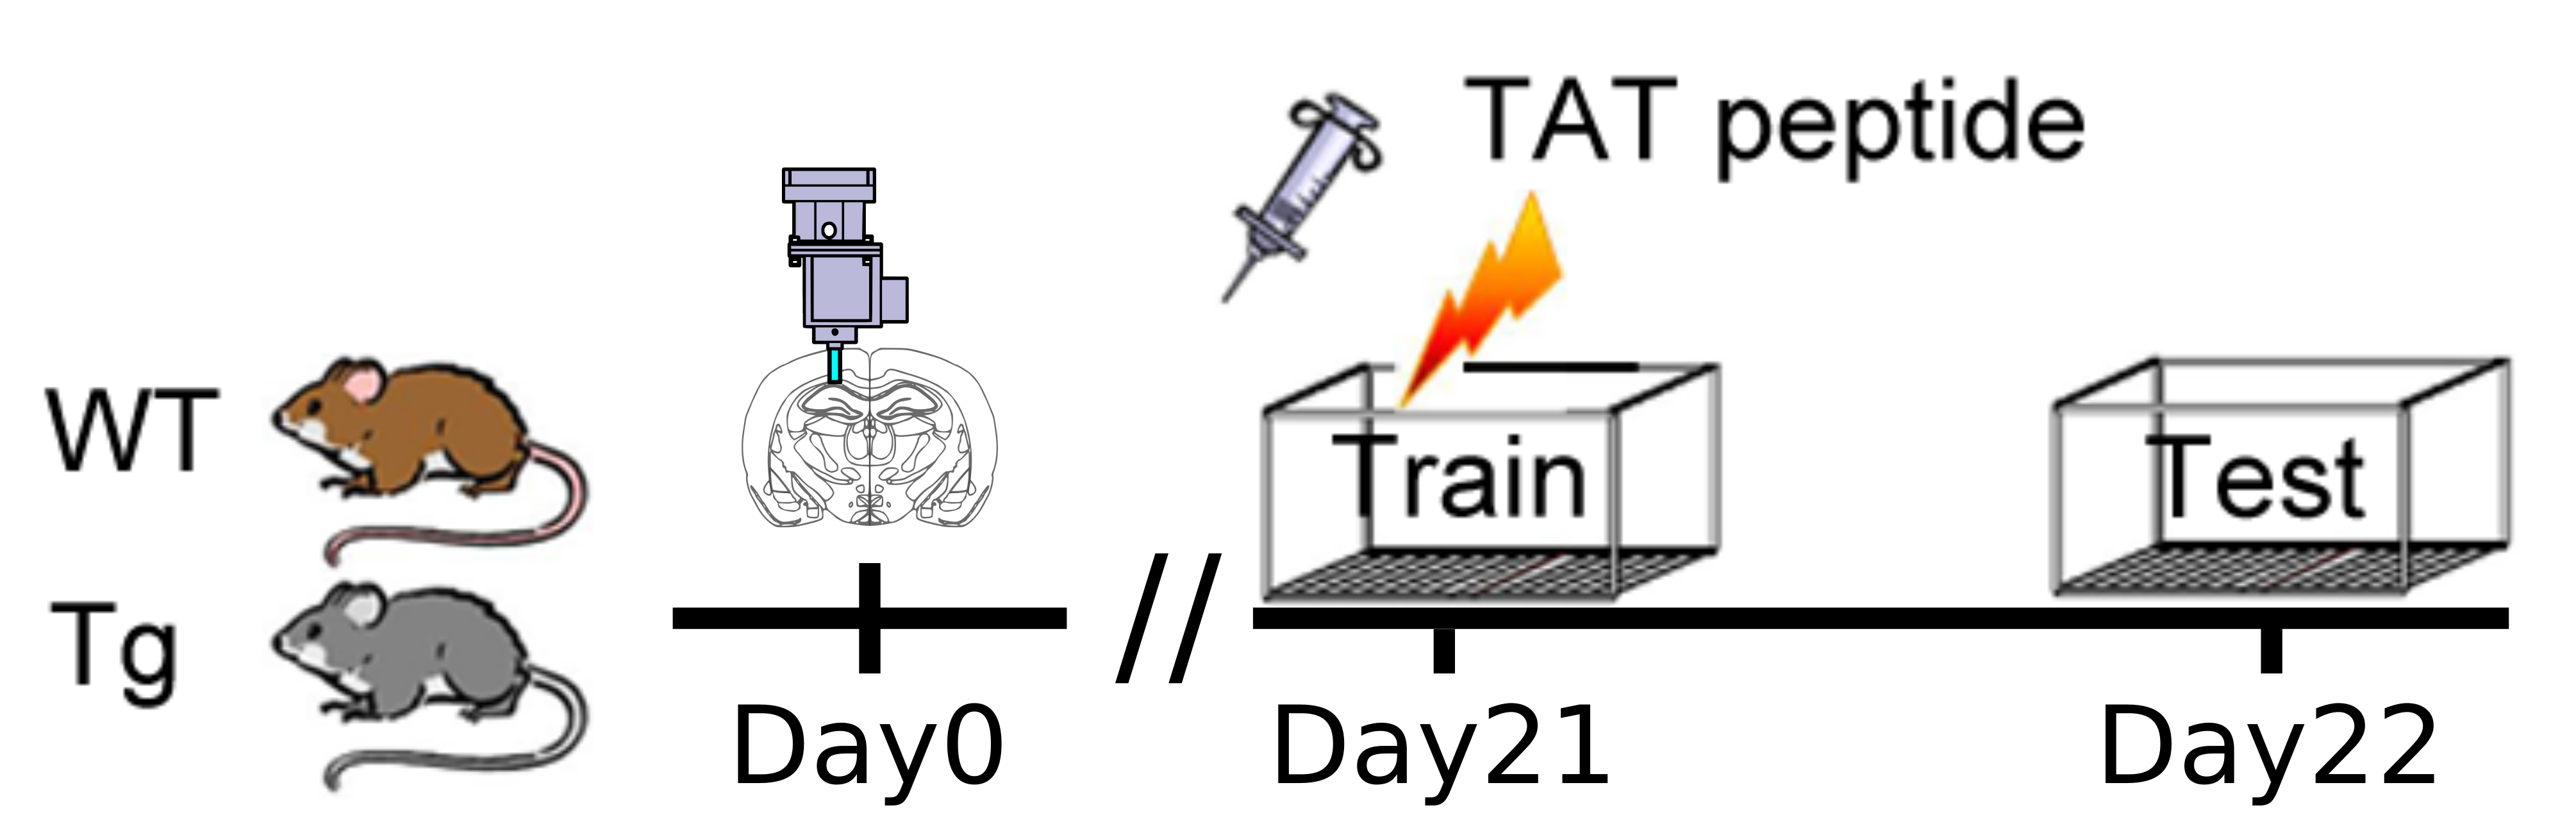
\includegraphics[width=\textwidth]{paradigm.png}
    \caption{Experimental paradigm. Adult \gls{wt} and \gls{tg} mice (with gCaMP6f expression) were implanted with a mini-microscope base-plate targeting CA1 hippocampus on day 0. The cells were visible three weeks later. Mice received \tglu peptide (i.p.) \SI{1}{\hour} before contextual fear conditioning. Mice were tested \SI{24}{\hour} later for freezing behaviour. Calcium transients were recorded for both training and testing session. \label{f.ad.paradigm}}
\end{figure}

\begin{figure}[h]
    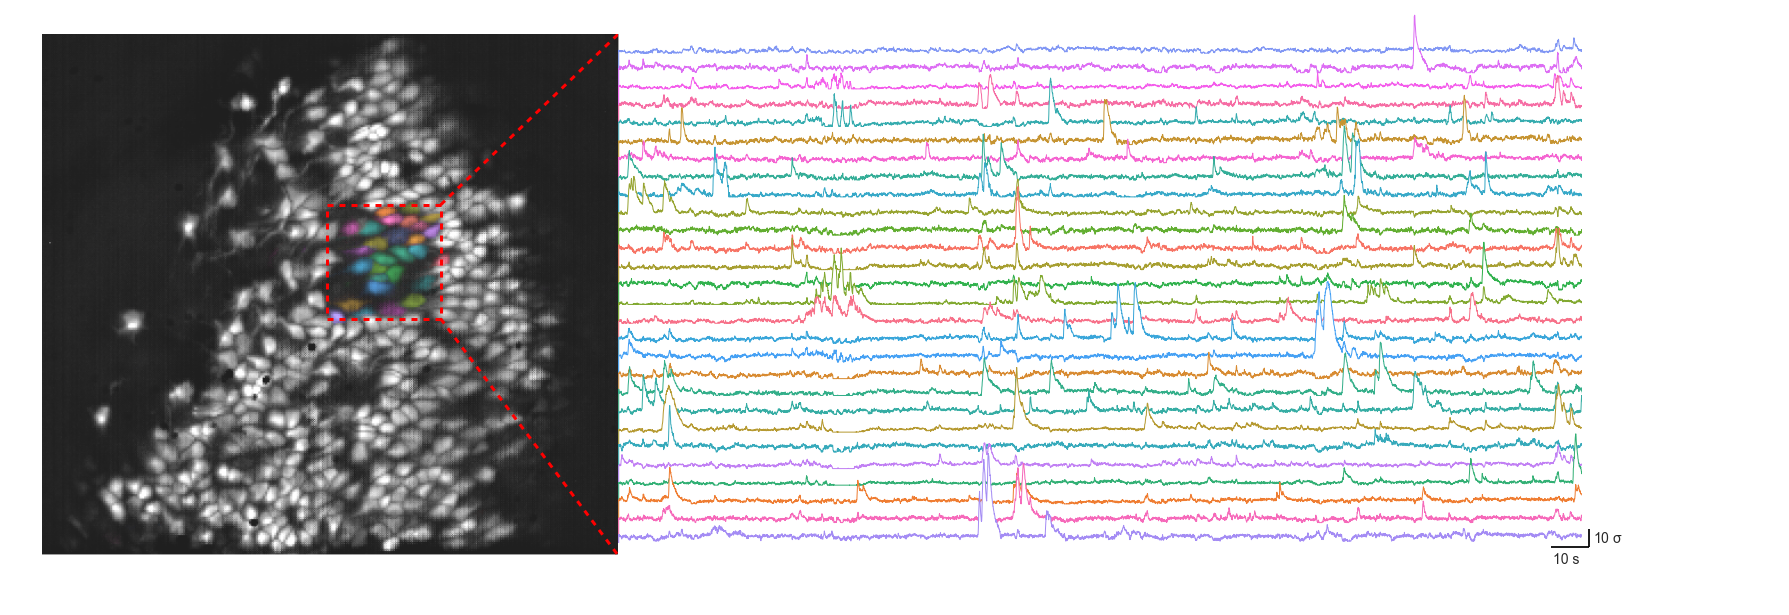
\includegraphics[width=\textwidth]{trace.png}
    \caption{Sample cell image and calcium transients. Transients are random coloured and correspond to cells of the same colour. \label{f.ad.trace}}
\end{figure}


Figure~\ref{f.ad.freezing} shows the percent of time spent freezing during the memory test. Two-way \gls{anova} has revealed a significant interaction between \textit{Genotype} and \textit{Treatment} (F\tsb{1,27}=5.45, p=0.027) as well as a significant main effect in \textit{Genotype} (F\tsb{1,27}=12.79, p=0.001).  \textit{Post hoc} tests show that \gls{tg}-Veh mice have significant lower freezing than \gls{wt} mice (\gls{wt}-Veh vs \gls{tg}-Veh, T=4.21, p<0.001), and this effect is fully rescued by \tglu treatment (\gls{tg}-\glu vs \gls{tg}-Veh, T=2.85, p=0.008; \gls{wt}-Veh vs \gls{tg}-\glu, T=1.12, p=0.27). \tglu has no significant effect on \gls{wt} mice (\gls{wt}-Veh vs \gls{wt}-\glu, T=0.355, p=0.72). 

This result is consistent with previous report \todo{cite} that the \gls{tg} mice have deficits in hippocampal-related memory tasks. It also confirms our hypothesis that the memory deficit of \gls{tg} mice can be rescued by \tglu treatment. 

\todo{freezing}
\begin{figure}[h]
    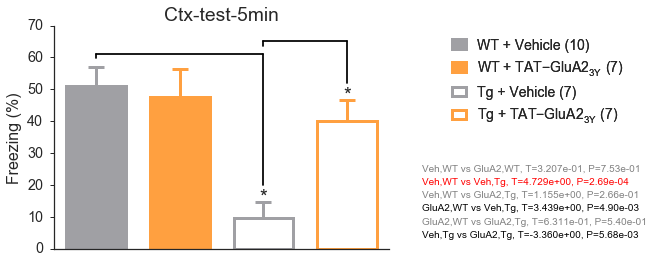
\includegraphics[width=\textwidth]{freezing.png}
    \caption{Percent of freezing during testing. \Gls{tg} mice have significant lower freezing, and \tglu treatment returns the freezing to wild-type level. \label{f.ad.freezing}}
\end{figure}

\subsection{\Gls{tg} mice can initiate freezing}
We then investigated whether the deficits in \gls{tg} mice is due to less freezing initiation or freezing maintenance. \todo{intro}

Figure~\ref{f.ad.freezing_profile} summarizes the number and length of freezing bouts in each group. There is no significant difference between groups in the number of freezing bouts (Figure~\ref{f.ad.freezing_freq}, omnibus F\tsb{3,27}=0.84, p=0.48). We then examined the average length of freezing bouts per mouse, and found a significant interaction between \textit{Genotype} and \textit{Treatment} (F\tsb{1,27}=6.5, p=0.01) and significant main effect of \textit{genotype} (F\tsb{1,27}=17.7, p<0.001). \textit{Post hoc} tests shows Tg-Veh mice have significantly shorter freezing bouts (WT-Veh vs Tg-Veh, T=4.75, p<0.001), and this deficit is fully rescued by \tglu treatment (Tg-\glu vs Tg-Veh, T=3.10, p=0.002; WT-Veh vs Tg-\glu, T=1.66, p=0.10). There is no effect of \tglu on \gls{wt} mice (T=0.22, p=0.83). This result suggest that the vehicle treated \gls{tg} mice do not have a deficit in initiating the freezing behaviour, however are unable to maintain freezing period for a longer time. 

\begin{figure}[h]
    \begin{subfigure}[h]{\textwidth}
        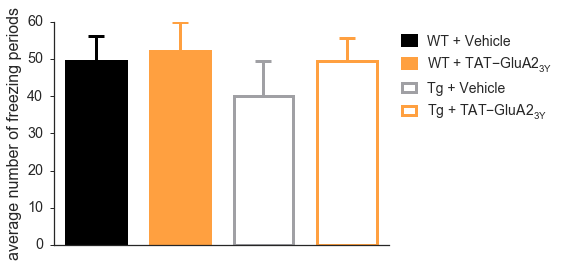
\includegraphics[width=\textwidth]{freezing_frequency.png}
        \caption{\label{f.ad.freezing_freq}}
    \end{subfigure}
    \begin{subfigure}[h]{\textwidth}
        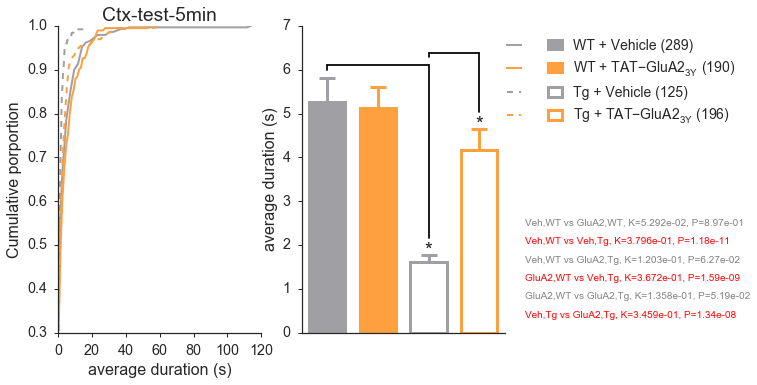
\includegraphics[width=\textwidth]{freezing_length.png}
        \caption{\label{f.ad.freezing_length}}
    \end{subfigure}
    \caption{Average number of freezing bouts \subref{f.ad.freezing_freq} and length of freezing bouts \subref{f.ad.freezing_length}. \Gls{tg} mice freeze as often as \gls{wt} mice, but with less duration. This is rescued by \tglu treatment. \label{f.ad.freezing_profile}}
\end{figure}


\subsection{\tglu rescues hyperactivity in \gls{tg} cells}

It has been known that amygloid plaques in \gls{tg} mice disturbs the excitatory-inhibitory balance of cells \todo{cite}. In the hippocampus \gls{ca1}, previous reports have found cells to be hyperactive in mouse model of \gls{ad}. Here we asked whether \gls{ca1} cells in \gls{tg} mice show hyperacitivity, and hypothesized that \tglu treatment is able to rescue the hyper-excitable phenotype.

Figure~\ref{f.ad.acttrain} shows average cell activity during training session before foot-shock. During training, two-way \gls{anova} reveals a significant interaction between \textit{Genotype} and \textit{Treatment} (F\tsb{1,3033}=7.7, p=0.006), as well as significant major effects of \textit{Genotype} (F\tsb{1,3033}=6.2, p=0.01) and \textit{Treatment} (F\tsb{1,3033}=5.1, p=0.02). \textit{Post hoc} tests shows that \gls{tg}-Veh has significantly higher cell activity (WT-Veh vs Tg-Veh, T=-3.72, p<0.001), and \tglu treatment is able to restore average cell activity to \gls{wt} level. (Tg-\glu vs Tg-Veh, T=-3.58, p<0.001; WT-Veh vs Tg-\glu, T=0.14, p=0.89). \tglu does not have any effect on \gls{wt} mice (WT-Veh vs WT-\glu, T=-0.137, p=0.89) This result is consistent with previous reports in the literature \citep{verret12}, showing cells in Tg mice have increase overall cell activity. Interestingly, while \tglu treatment restores the mean cell activity during training, the distribution of cell activity is significantly different from \gls{wt} (WT-Veh vs Tg-\glu, K=0.16, p<0.001). As is shown in the cumulative distribution plot, Tg-\glu still have a over-proportion of highly active cells. 
\todo{In Discussion: \tglu is not able to rescue cells with very high activity}

Similar effect were found during testing (Figure~\ref{f.ad.acttest}). Two-way \gls{anova} revealed significant interaction of \textit{Genotype} and \textit{Treatment}(F\tsb{1,3029}=78.4, p<0.001), as well as major effects of \textit{Genotype} (F\tsb{1,3029}=32.7, p<0.001) and \textit{Treatment} (F\tsb{1,3029}=27.4, p<0.001). \textit{Post hoc} tests show significant increase of cell activity in Tg-Veh group (WT-Veh vs Tg-Veh, T=-10.1, p<0.001), and this effect is corrected by \tglu treatment (WT-Veh vs Tg-\glu, T=0.73, p=0.47; Tg-\glu vs Tg-Veh, T=-9.97, p<0.001). There is also a trend of increase in cell activity after \tglu treatment in \gls{wt} group, however the p-value is close to threshold after correction of multiple comparison (WT-Veh vs WT-\glu, T=-2.53, p=0.012, threshold = 0.013). Interestingly during testing, \tglu is able to fully rescue the hyper-activity in \gls{tg} group (\gls{kstest}: Veh-WT vs Tg-\glu, K=0.06, p=0.07; Tg-Veh vs Tg-\glu, K=2.29, p<0.001). These results suggest that the effect \tglu treatment is a long-lasting effect: treatment during memory encoding is also able to rescue \gls{ca1} hyperactivity in \gls{tg} mice during memory test \SI{24}{\hour} later.

Comparing the cell activity between testing and training, we found that the \gls{tg} mice have significantly increased cell activity during testing,  which is not found in \gls{wt} mice (Figure~\ref{f.ad.actdiff}; Two-way \gls{anova}, \textit{Genotype} $\times$ \textit{Treatment} interaction F\tsb{1,4380}=32.4, p<0.001, \textit{Genotype} main effect F\tsb{1,4380}=23.0, p<0.001, \textit{Treatment} main effect F\tsb{1,4380}=23.6, p<0.001; \textit{post hoc} test WT-Veh vs Tg-Veh, T=-7.4, p<0.001, WT-Veh vs WT-\glu, T=-0.487, p=0.63). \tglu treatment blocks the increase of the cell activity during testing (Tg-\glu vs Tg-Veh, T=-7.5, p<0.001). The cumulative plot suggests that \gls{tg} mice have similar proportion of cells with increased activity, however in \gls{tg} mice the cells increased more than those in \gls{wt} mice. This result confirms of previous report that mouse model of \gls{ad} show disrupted excitation-inhibition balance in \gls{ca1} \citep{palop16}.

\begin{figure}[h]
    \begin{subfigure}[h]{\textwidth}
        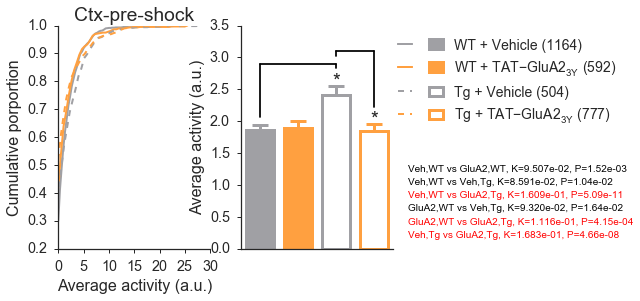
\includegraphics[width=\textwidth]{activity_train.png}
        \caption{\label{f.ad.acttrain}}
    \end{subfigure}
    \begin{subfigure}[h]{\textwidth}
        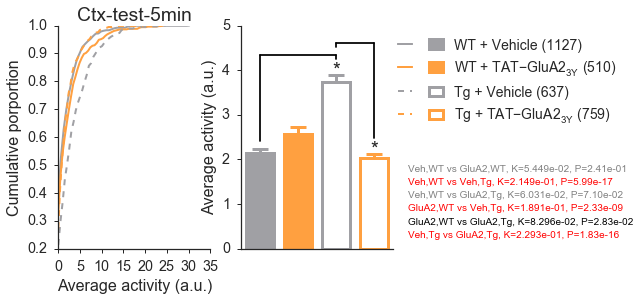
\includegraphics[width=\textwidth]{activity_test.png}
        \caption{\label{f.ad.acttest}}
    \end{subfigure}
    \caption{Distribution and mean of average cell activity during \subref{f.ad.acttrain} training before footshock and \subref{f.ad.acttest} memory test. Cells in the Tg mice are significantly more active, and this is rescued by \tglu treatment. Cell numbers are listed in the legend with paranthesis. The cell activity are measured in \gls{au}. \label{f.ad.activity}}
\end{figure}

\begin{figure}[h]
    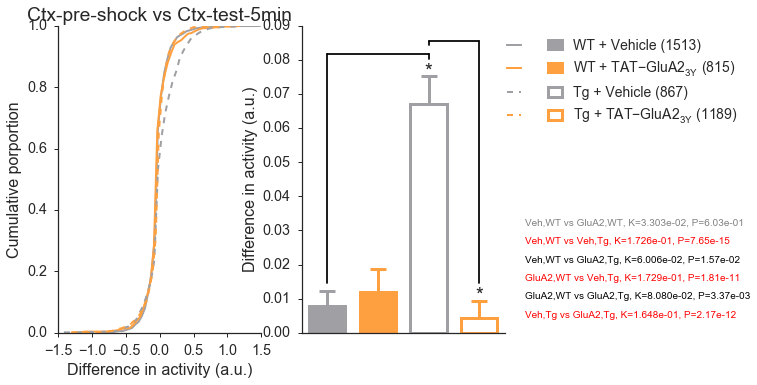
\includegraphics[width=\textwidth]{diff_activity.png}
    \caption{Cell activity difference between training and testing sessions. \gls{tg} mice significantly increased their cell activity during testing session, and this is blocked by \tglu treatment. \label{f.ad.actdiff}}
\end{figure}


\subsection{\tglu rescues contextual fear memory recall by decreasing activity}

We then investigated the average cell activity when the mice were freezing or not freezing during the 5-min context memory test. \todo{refer to literature}. The result is summarized in figure~\ref{f.ad.activity_freezing}.  

Two-way \gls{anova} on the average activity when mice are freezing shows insignificant interaction between \textit{Genotype} and \textit{Treatment} (F\tsb{1,3034}=-0.03, p=0.97). There is significant main effect in both \textit{Genotype} (F\tsb{1,3034}=6.9, p=0.008) and \textit{Treatment} (F\tsb{1,3034}=18.7, p<0.001). \Gls{tg} mice show significantly increased activity during freezing, and \tglu treatment has a significant inhibitory effect on cell activity. \todo{discuss about highly active cells in the cumulative distribution plot}

For the cell activity when the mice did not show freezing behaviour, we performed two-way \gls{anova}, and found a significant \textit{Genotype} $\times$ \textit{Treatment} interaction (F\tsb{1,3029}=13.6, p<0.001), as well as a significant main effect of \textit{Treatment} (F\tsb{1,3029}=12.3, p<0.001). \tglu treatment only significantly decreased activity in the \gls{tg} mice (Tg-\glu vs Tg-Veh, T=-5.4, p<0.001), and have no effect on \gls{wt} mice \todo{stats}. These results suggest \tglu may rescue the \gls{tg} phenotype by globally decreasing background cell activity.These results suggest \tglu treatment is able to decrease cell activity during freezing for both \gls{tg} and \gls{wt} mice, however it also decrease cell activity in gls{tg} when the mouse is not freezing.


\begin{figure}[h]
    \begin{subfigure}[h]{\textwidth}
        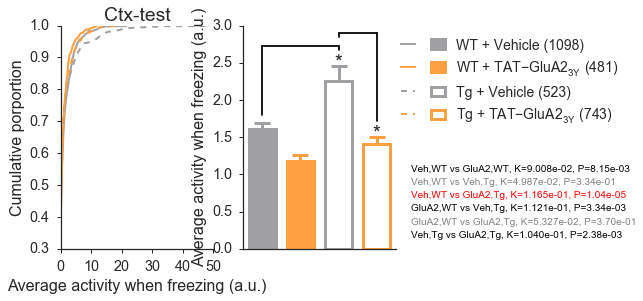
\includegraphics[width=\textwidth]{activity_freezing.png}
        \caption{\label{f.ad.actf}}
    \end{subfigure}
    \begin{subfigure}[h]{\textwidth}
        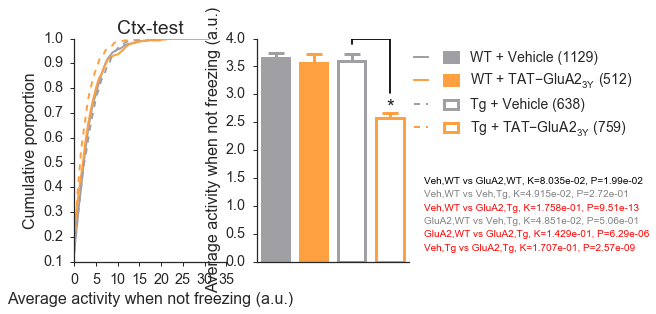
\includegraphics[width=\textwidth]{activity_moving.png}
        \caption{\label{f.ad.actnf}}
    \end{subfigure}
    \caption{Average cell activity when the mice was \subref{f.ad.actf} freezing and \subref{f.ad.actnf} not freezing during the 5-min contextual memory test. Cells in \gls{tg} mice have significantly higher activity during freezing, and \tglu treatment decreases cell activity in both \gls{wt} and \gls{tg} groups. When the mice were not freezing, \tglu treatment decreases cell activity only in \gls{tg} mice, but have no effect in \gls{wt} mice. This result suggests that the effect of \tglu in \gls{tg} mice is a global decrease of cell activity. \label{f.ad.activity_freezing}}
\end{figure}
\begin{comment}
\begin{figure}[h]
    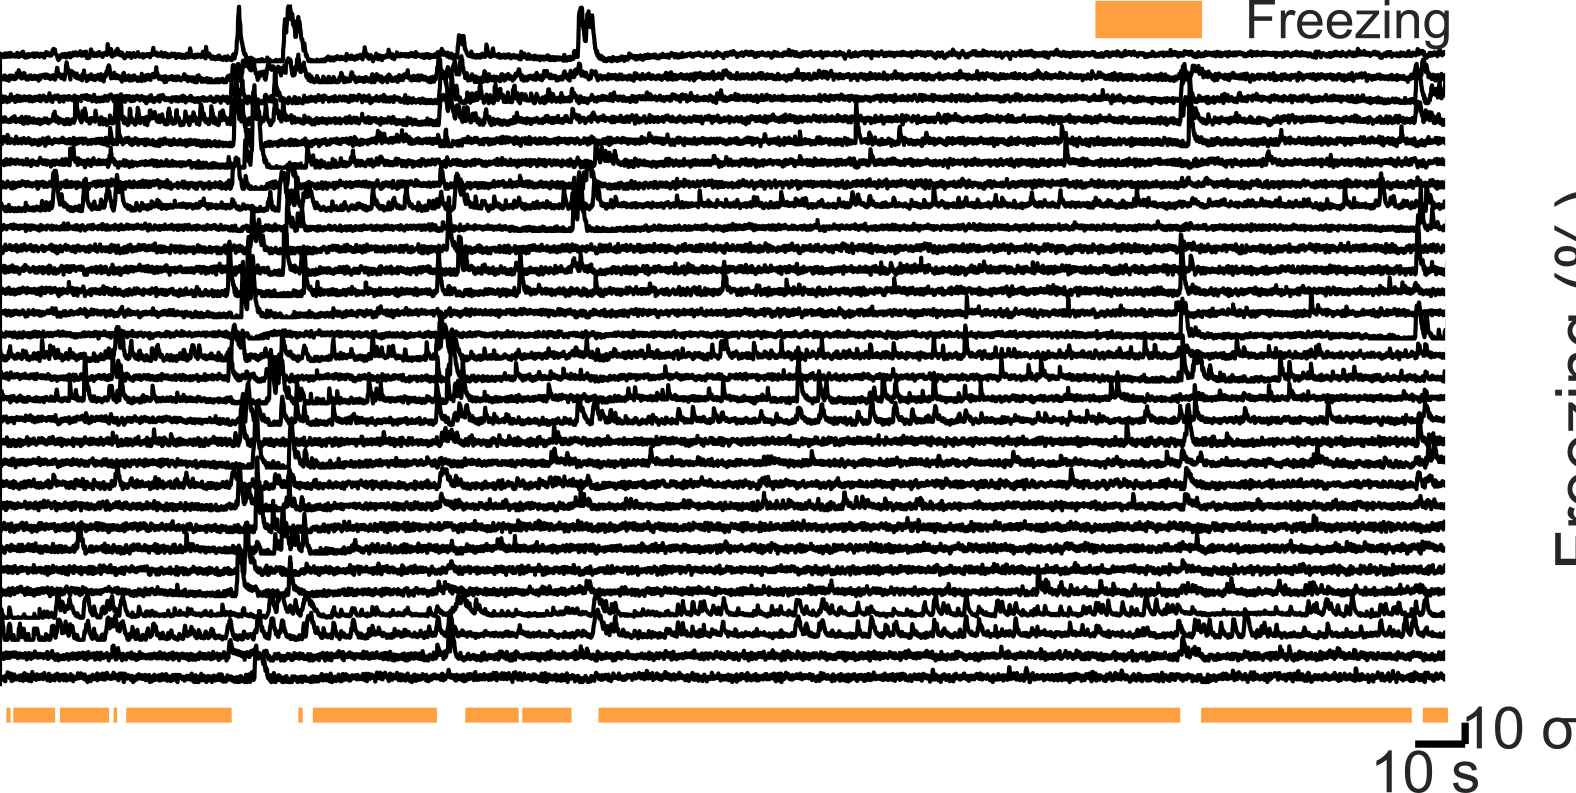
\includegraphics[width=\textwidth]{sample_trace.png}
    \caption{Sample calcium transients from cells with highest freezing information in a mouse. It appears that cells encode freezing by decreasing their activity. \label{f.ad.sample_trace}}
\end{figure}
\begin{figure}[h]
    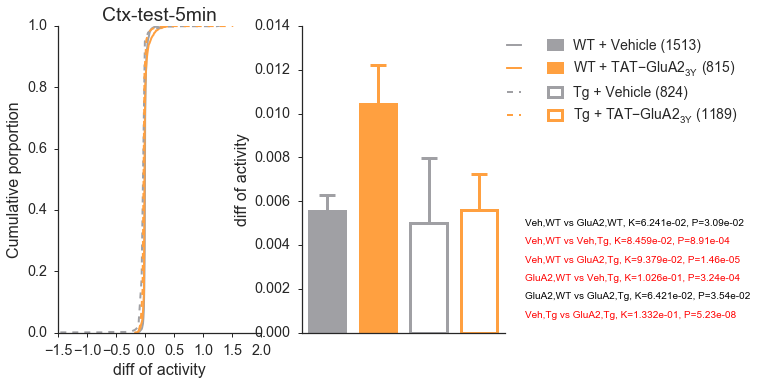
\includegraphics[width=\textwidth]{ch_activity.png}
    \caption{Distribution and mean of activity difference between not-freezing and freezing. This confirms the intuition from Figure~\ref{f.ad.sample_trace} that most of the cells decrease activity during freezing. \label{f.ad.ch_activity}}
\end{figure}
\end{comment}

\subsection{\tglu rescues freezing encoding deficit in \gls{tg} cells}

Previous reports have suggested that \gls{ca1} neurons in \gls{tg} mice have deficits encoding spatial information \todo{cite ji}. We then investigated how \gls{wt} and \gls{tg} cells encodes freezing.  \todo{intro}

First we looked at cells individually, and calculated the mutual information between the calcium transient and freezing \citep{ross14, victor02}. Mutual information captures both linear and non-linear relationship between two random variables and reflects how much prediction power one variable has for another. Following the naming from \citet{skaggs93}, where the mutual information between cell activity and animal's position is dubbed ``spatial information'', here we refer to the mutual information between cell activity and mouse's freezing behaviour as ``freezing information''. 

The group differences in freezing information was compared using two-way \gls{anova}. There is a significant \textit{Genotype} $\times$ \textit{Treatment} interaction (F\tsb{1,4380}=126.7, p<0.001), as well as main effects in both \textit{Genotype} (F\tsb{1,4380}=254.0, p<0.001) and \textit{Treatment} (F\tsb{1,4380}=54.7, p<0.001). \textit{Post hoc} tests show Tg-Veh group has significantly less freezing information (WT-Veh vs Tg-Veh, T=19.3, p<0.001), and this deficit is partially rescued by \tglu treatment (Tg-\glu vs Tg-Veh, T=13.2, p<0.001), as Tg-\glu group has significantly less freezing information than WT-Veh group (WT-Veh vs Tg-\glu, T=6.0, p<0.001; Figure~\ref{f.ad.freeze_info}). WT-\glu has significantly less freezing information than WT-Veh, although the significance is close to threshold (WT-Veh vs WT-\glu, T=2.5, p=0.011, threshold=0.013). This result suggests in the \gls{tg} group, the individual cell activity in hippocampus \gls{ca1} is not a good predictor of the mouse's freezing behaviour. This is partially recovered by \tglu treatment. 
\begin{figure}[h]
    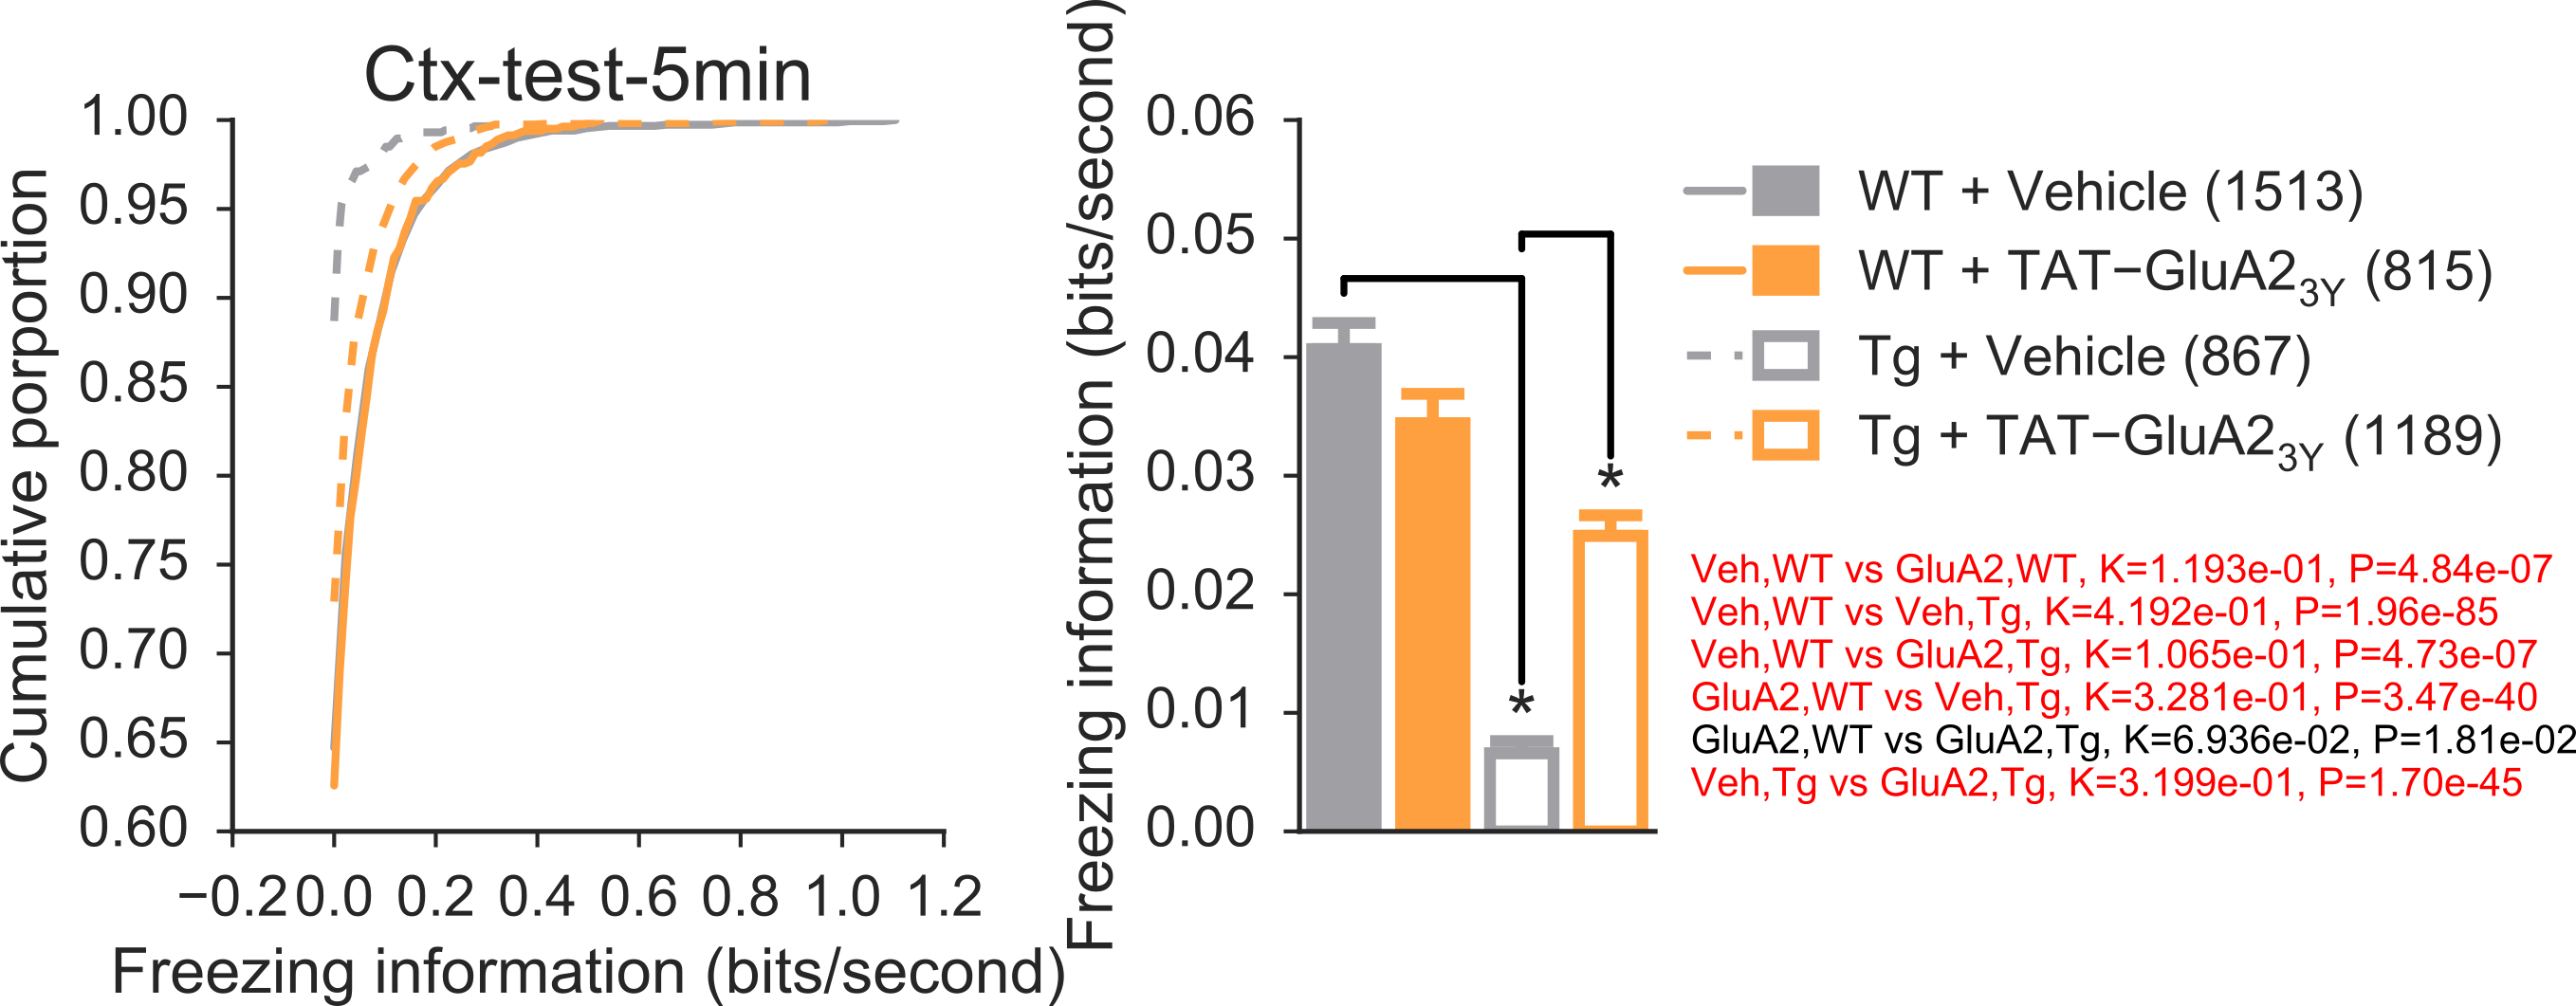
\includegraphics[width=\textwidth]{freeze_info.png}
    \caption{Freezing information during the context memory test. This measurement represent how much information a particular cell have in a period of time about whether the mouse is freezing. Cells in \gls{tg} mice encode significantly less freezing information than the \gls{wt} groups, and \tglu treatment can only partially rescue the effect. \label{f.ad.freeze_info}}
\end{figure}
    

%\subsection{Deficit of freezing encoding in \gls{tg} animals is not a result of animal's position or freezing levels}

Given that CA1 cells are known to encode place, and \gls{tg} mice have deficits in spatial encoding, it is possible the difference of spatial encoding confounded the freezing information measurement. Moreover, \gls{tg} mice have low level of freezing during the memory test. It is possible that mice with low level of freezing, therefore weaker memory, have deficits freezing encoding in the cells. That is, the difference of freezing information in \gls{tg} is a result of weaker memory instead of a specific deficit due to the expression of the transgene. To eliminate the effect of the mouse's position, we have calculated the average freezing information for all mouse positions, therefore eliminating the contribution of place. To control for the potential effect of freezing level, we have included it as a covariate in the two-way \gls{anova}. 

The result is similar to the freezing information observed in Figure~\ref{f.ad.freezing_info} (Figure~\ref{f.ad.freeze_ctrl}). There is a significant interaction between \textit{Genotype} and \textit{Treatment} (F\tsb{1,4380}=97.9, p<0.001), as well as significant main effects in \textit{Genotype} (F\tsb{1,4380}=139.4, p<0.001) and \textit{Treatment} (F\tsb{1,4380}=100.3, p<0.001). Furthermore, this test revealed that mice's freezing level is not a significant confounding factor (T=-0.65, p=0.50) for freezing information. And again, \textit{post hoc} tests show that Tg-Veh has significant lower freezing information with position controlled (WT-Veh vs Tg-Veh, T=15.1, p<0.001), and fully rescued by \tglu (Tg-\glu vs Tg-Veh, t=13.9, p<0.001; WT-Veh vs Tg-\glu, t=1.9, p=0.06, threshold=0.013). This result suggest that the deficit of freezing encoding in \gls{tg} is independent of the mouse's position in space and freezing levels during the memory test session.
\begin{figure}[h]
    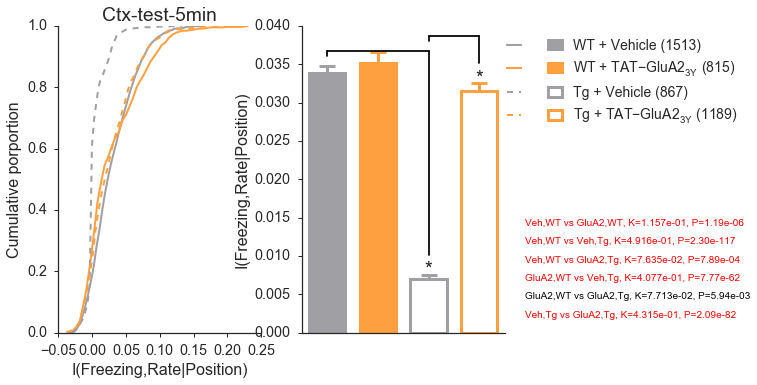
\includegraphics[width=\textwidth]{freeze_position.png}
    \caption{Freezing information encoded in cells is not reliant on mice's position or freezing level. This measurement removes the effect of position from freezing information measurement. This result is similar to Figure~\ref{f.ad.freeze_info}. This suggest that the position of the mouse is not a confounding factor for freezing information measurement. \label{f.ad.freeze_ctrl}}
\end{figure}

\begin{comment}

An additional potential confound comes from the mouse's behaviour. Within \gls{wt} mice, there is a significant correlation between freezing information and freezing \todo{stats and figure}. Given that \gls{tg} mice do not freeze well during testing, we ask is the encoding deficit found in \gls{tg} mice explained by the correlation of freezing and encoding? To investigate this question, we added freezing as a covariate into the two-way \gls{anova} model for position-controlled freezing information. The resulting model shows while percent of freezing is a significant confound in measuring freezing information (F\tsb{1,4379}=42.0, p<0.001), there is still significant major effect of genotype (F\tsb{1,4379}=34.0, p<0.001) and treatment (F\tsb{1,4379}=6.7, p=0.009), as well as a significant interaction between the two factors (F\tsb{1,4379}=5.6, p=0.017). Similarly to Figure~\ref{f.ad.freeze_ctrl}, \textit{Post hoc} tests have found a significant decrease of freezing information in Tg-Veh with freezing level controlled (WT-Veh vs Tg-Veh, t=5.46, p<0.001), as well as a partial rescue by \tglu treatment (Tg-\glu vs Tg-Veh, t=3.45, p=0.001; WT-Veh vs Tg-\glu, t=2.93, p=0.003). And again, no effect of \tglu on \gls{wt} mice (WT-Veh vs WT-\glu, t=-0.30, p=0.75). These results suggest that while freezing information is correlated with percent of freezing, \gls{tg} mice have additional deficit in encoding freezing, and this deficit is partially rescued by \tglu treatment. 

In addition, we also checked whether the freezing information coding is a result of different freezing or uneven spatial coverage of the behavioural chamber, which are represented by freezing entropy and spatial entropy respectively. To check these two factors, we have pooled the groups with similar behaviour (\gls{wt}, \gls{wt}-\tglu, \gls{tg}-\tglu), and correlated percent freezing, freezing entropy, total distance and spatial entropy against freezing information within the pooled groups. If the behavioural measurement have no influence in the freezing information, we would expect no correlation. Indeed, that is what we have found in Figure~\ref{f.ad.corrs}. These control measurements have shown that the reduction of freezing encoding in the Tg mice is not affected by the difference in the mice's behaviour.
\begin{figure}[h]
    \begin{subfigure}[t]{.5\textwidth}
        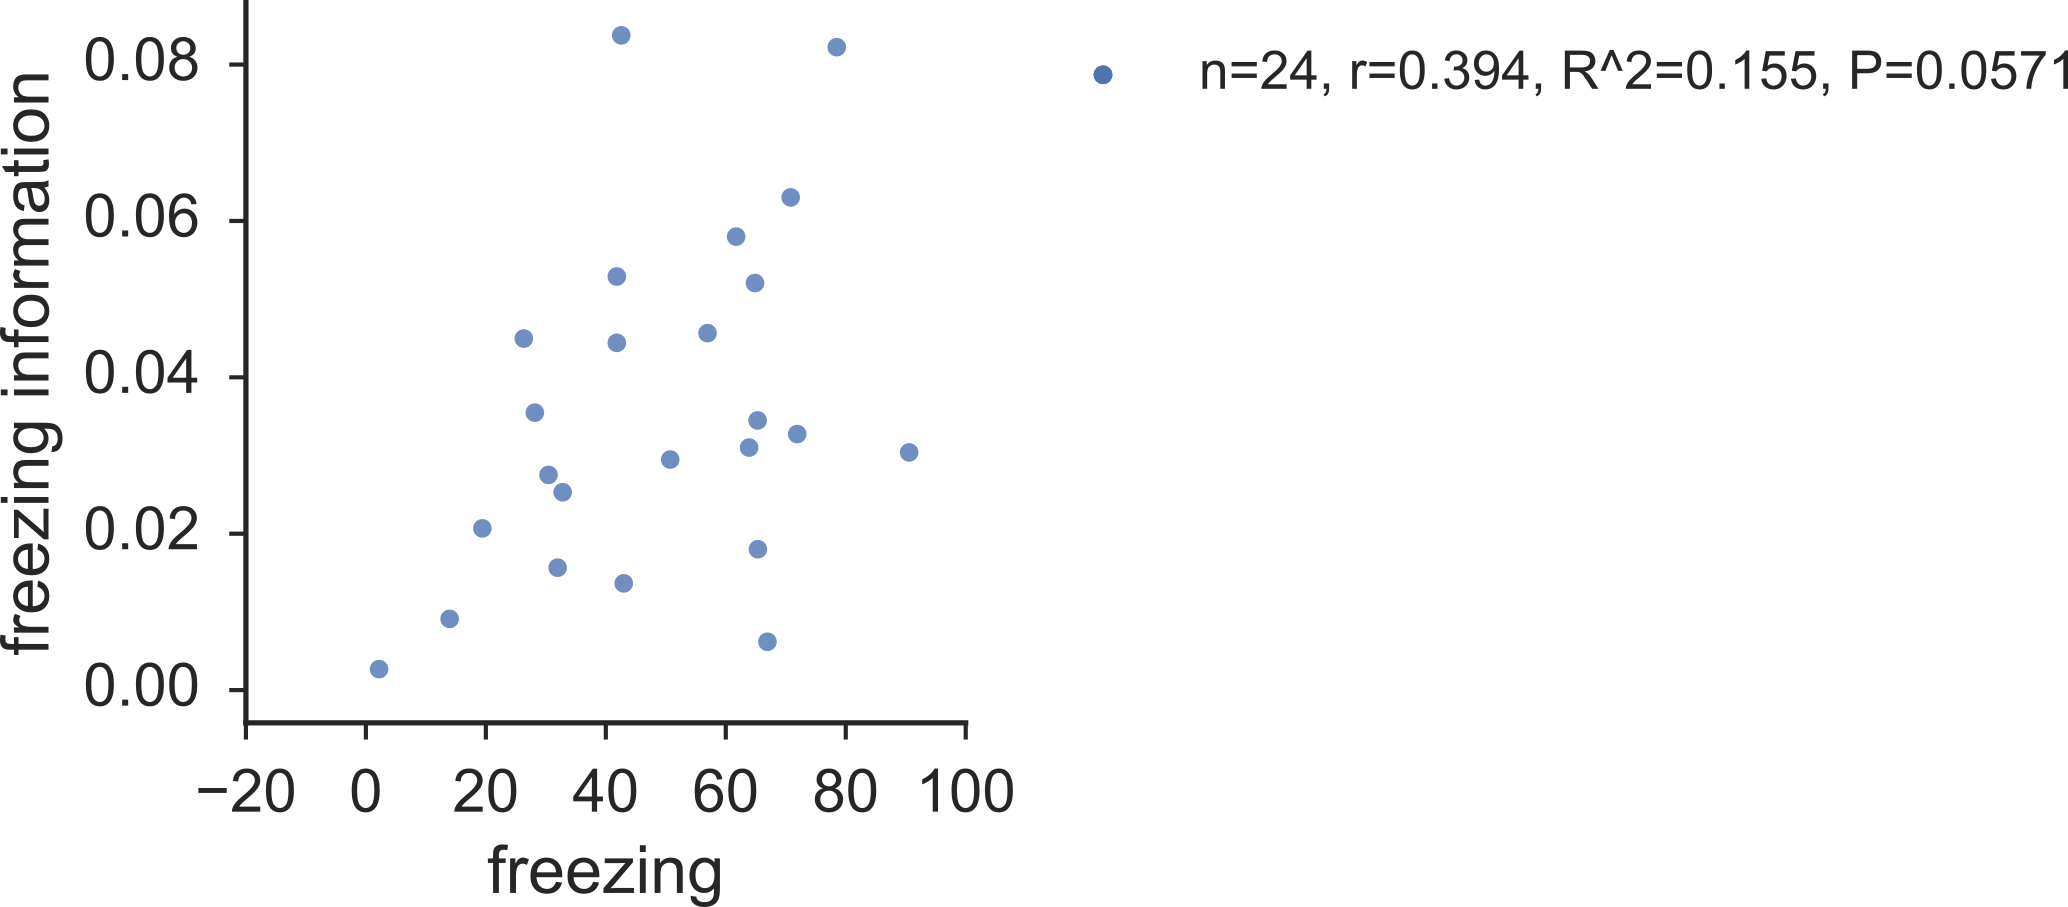
\includegraphics[width=\textwidth]{corr1.png}
        \caption{}
    \end{subfigure}
    \begin{subfigure}[t]{.5\textwidth}
        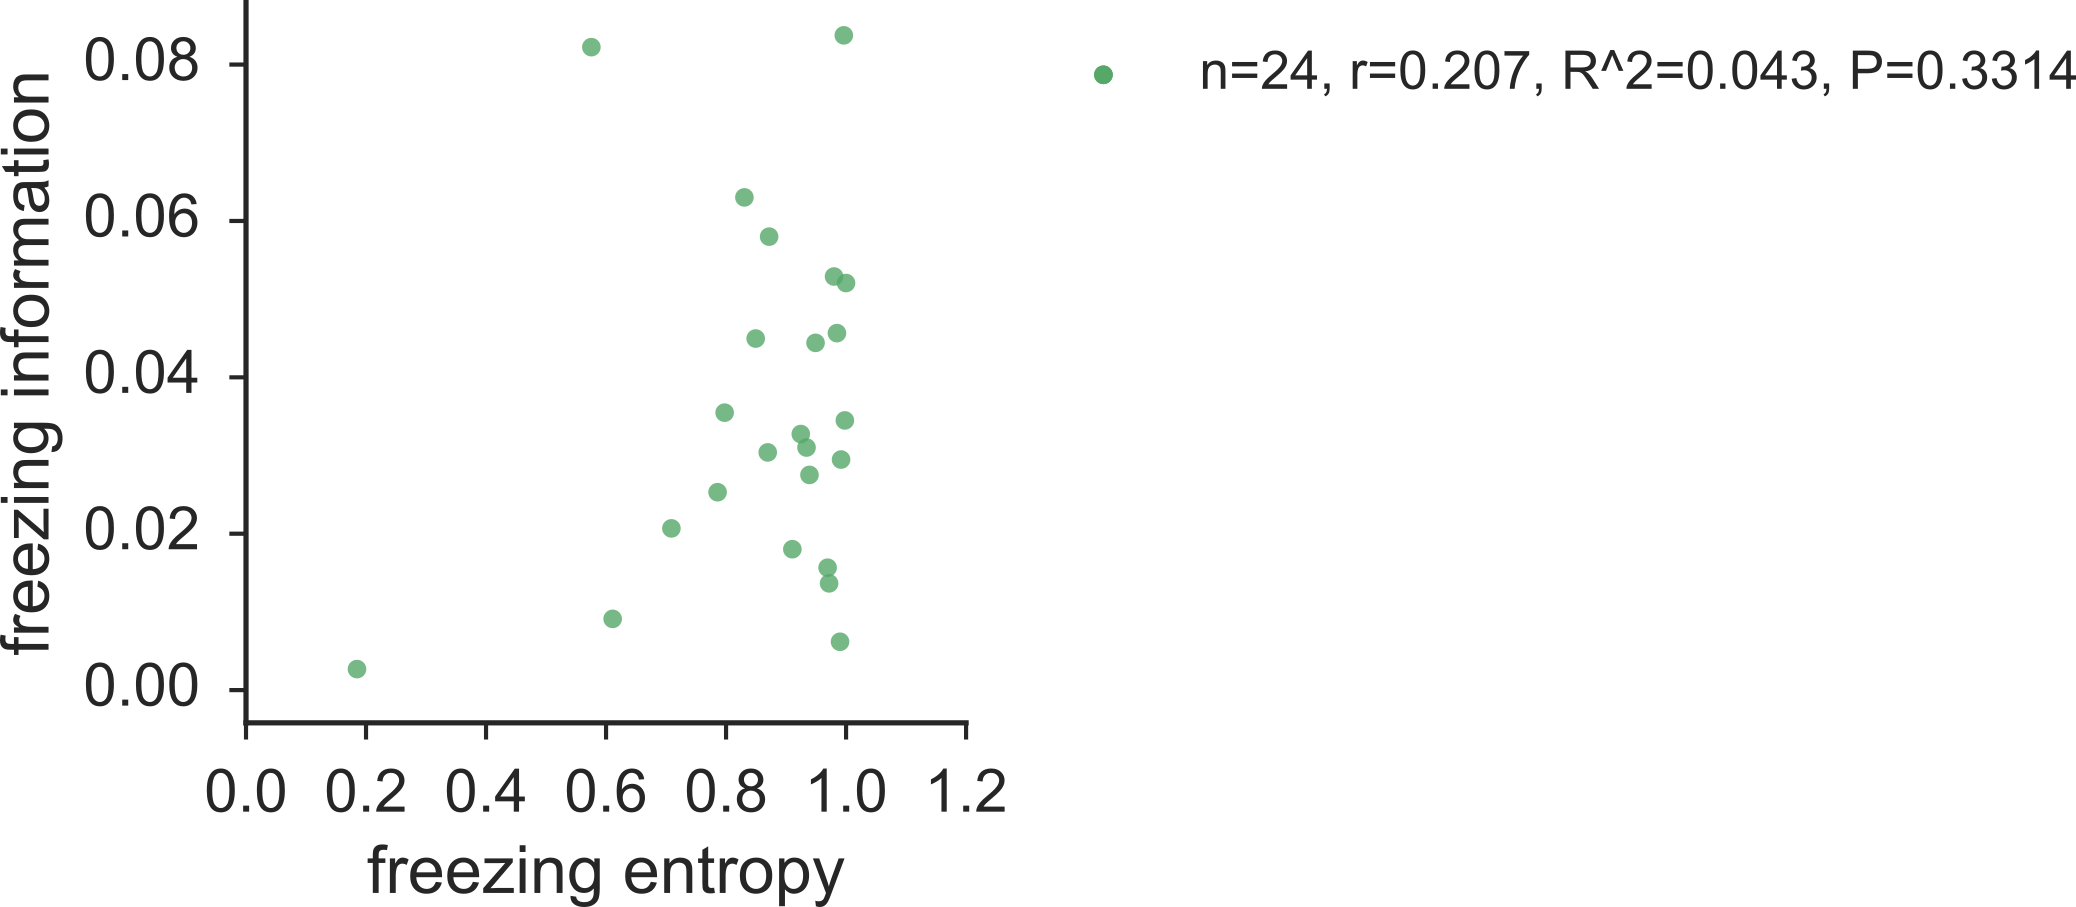
\includegraphics[width=\textwidth]{corr2.png}
        \caption{}
    \end{subfigure}
    \begin{subfigure}[t]{.5\textwidth}
        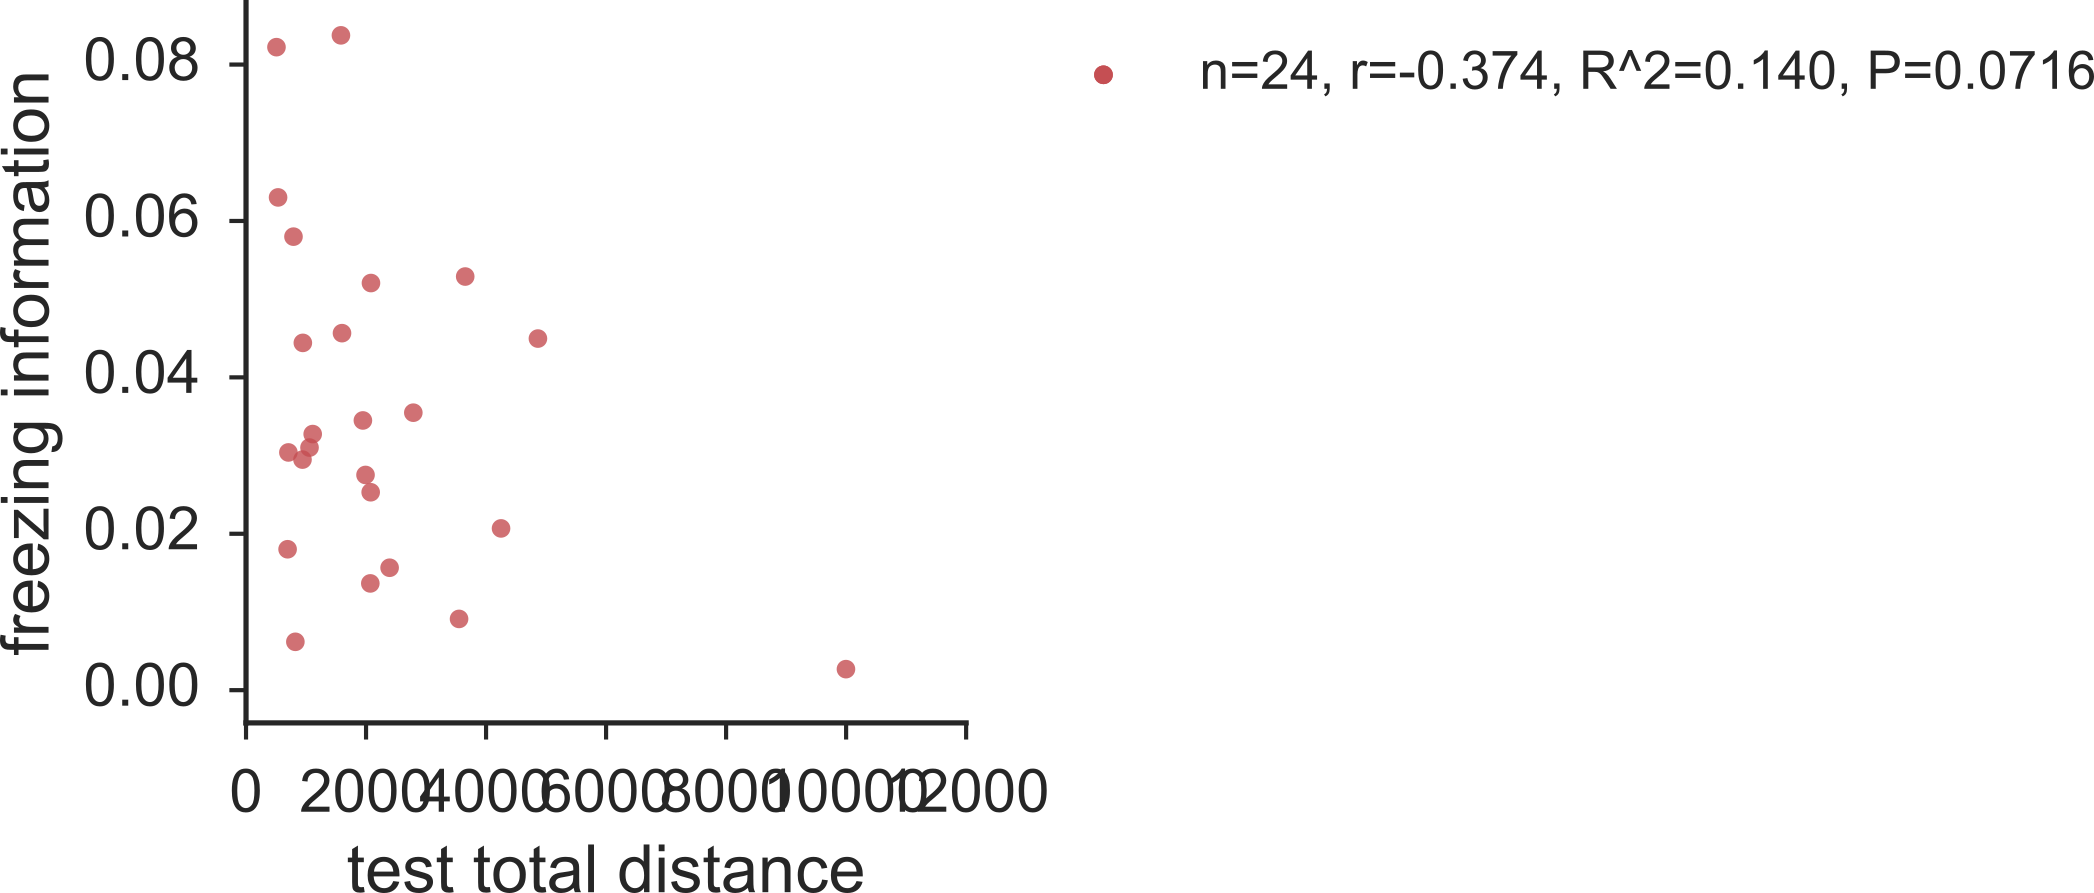
\includegraphics[width=\textwidth]{corr3.png}
        \caption{}
    \end{subfigure}
    \begin{subfigure}[t]{.5\textwidth}
        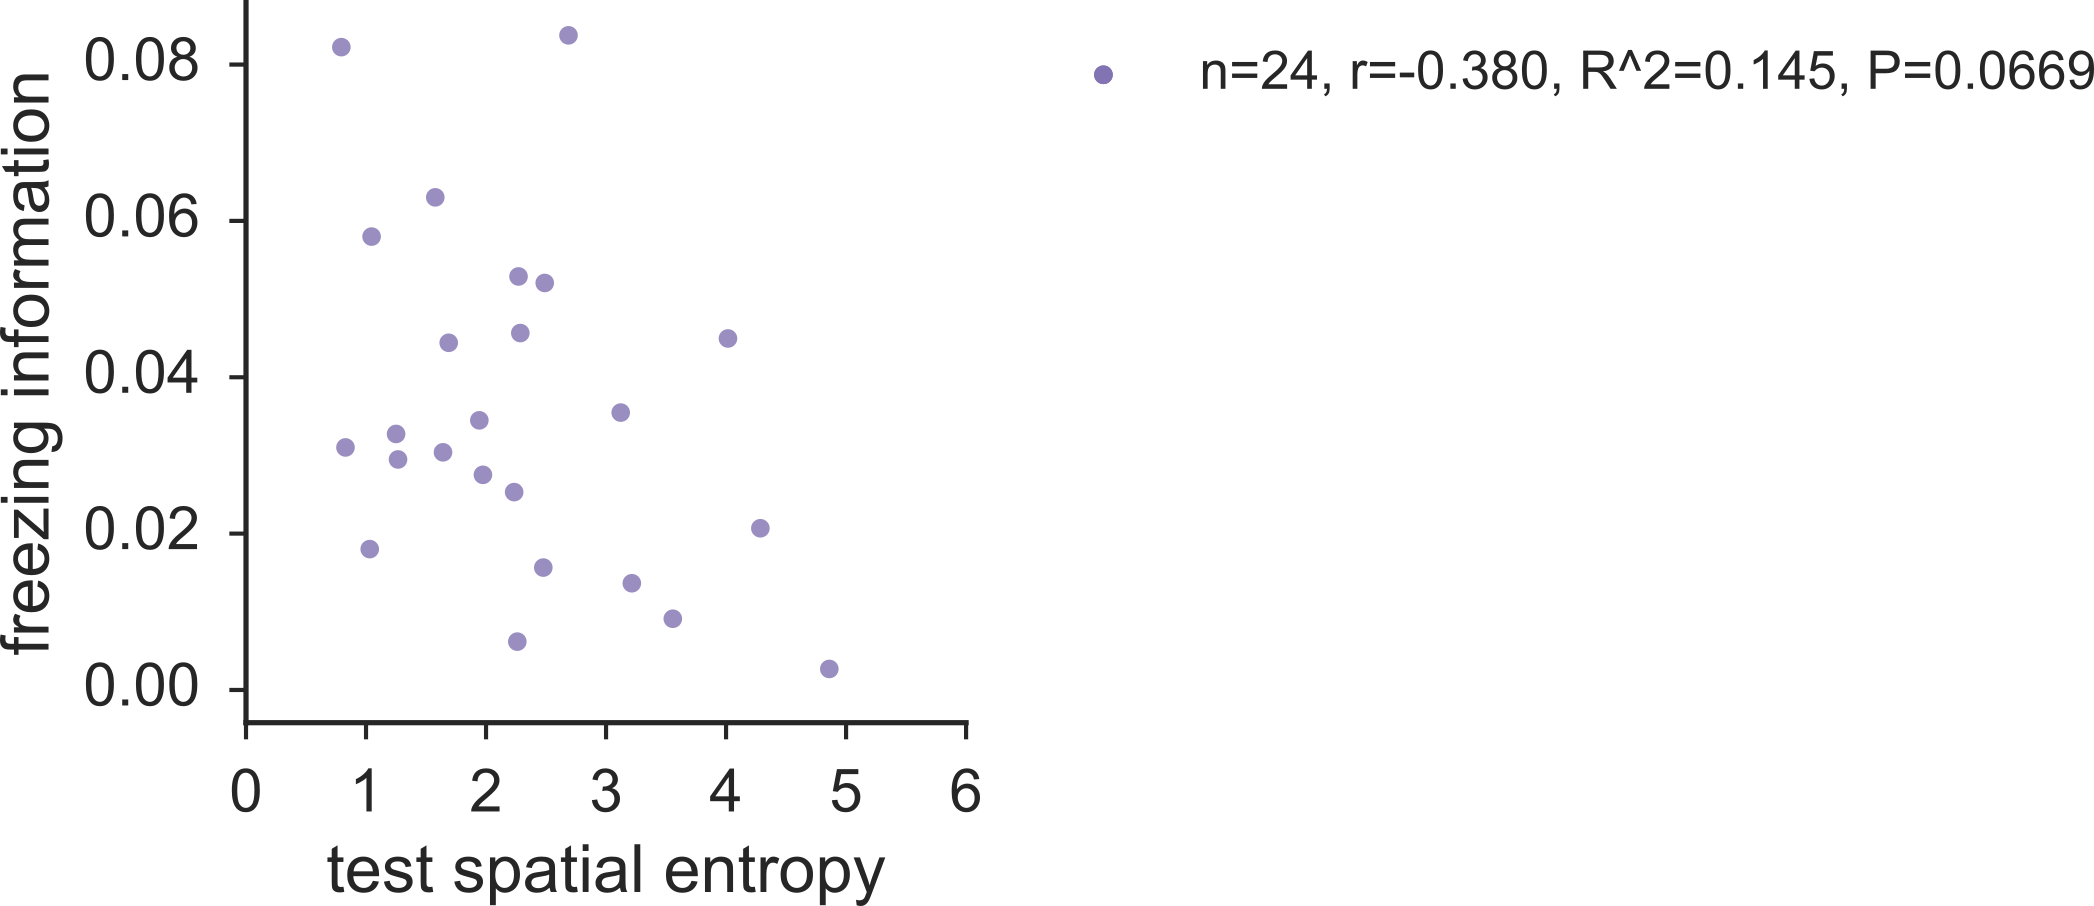
\includegraphics[width=\textwidth]{corr4.png}
        \caption{}
    \end{subfigure}
    \caption{Scatter plots of varies behaviour measurement against freezing information, in pooled \gls{wt}, \gls{wt}-\glu and \gls{tg}-\glu. Given there is no group difference between the three groups, if any of the behaviour factor is confounding, the it will contribute to within-group difference and correlate with freezing information. We have found no significant correlations. However the near significance of percent freezing and spatial entropy correlations will need further investigation. \label{f.ad.corrs}}
\end{figure}
\end{comment}



\subsection{Network encoding of freezing behaviour}

While all the measurements we have performed considers each cell individually, are the cells independent of each other, or is part of the information encoded in the coordination between them? \todo{relate to literature}

To answer this question, we took advantage of machine learning algorithms. A \gls{nbc} models the cells independent of each other, and therefore can use neural signatures in individual cells for prediction. A general classifier such as a \gls{gsvm} on the other hand, is able to take advantage of information encoded by individual cells as well as the ensemble of them. To investigate whether the neural signature of recalling a contextual fear memory (as measured by the freezing behaviour) is encoded by the cells individually or in the network, we trained both an \gls{nbc} and a \gls{gsvm} to predict freezing behaviour from the calcium transients at each time point. The performance of \gls{nbc} would represent prediction power encoded independently in cells, and the performance of \gls{gsvm} represents total prediction power of the network.

The result is shown in Figure~\ref{f.ad.classifier}. We calculated F1 score as a measurement of classifier performance, which considers both the precision and sensitivity of the classifier. A three-way \gls{anova} of \textit{Genotype} $\times$ \textit{Treatment} $\times$ \textit{Classifier} was carried out. We found a significant interaction between \textit{Genotype} and \textit{Treatment} (F\tsb{1,50}=14.2, p<0.001), as well as significant main effects of each factors (\textit{Genotype}, F\tsb{1,50}=15.6, p<0.001; \textit{Treatment} F\tsb{1,50}=5.5, p=0.02; and \textit{Classifier} F\tsb{1,50}=9.0, p=0.004). Since the \textit{Classifier} factor only have a significant major effect, for the \textit{post hoc} tests we used F-test to only compare different levels of \textit{Genotype} and \textit{treatment}. F1 score of Tg-Veh is significantly less than WT-Veh (F\tsb{2,50}=16.4, p<0.001), and this effect is rescued by \tglu treatment (Tg-\glu vs Tg-Veh, F\tsb{2,50}=9.7, p<0.001). There is no significant difference between WT-Veh and Tg-\glu (F\tsb{2,50}=0.63, p=0.54), and \tglu treatment has no significant effect on \gls{wt} group (WT-Veh vs WT-\glu, F\tsb{2,50}=0.20, p=0.81).  

These results show \gls{gsvm} significantly outperforms the \gls{nbc} classifier across all groups, suggesting that the network encodes more information about freezing than the cells individually. Moreover, both classifiers perform significantly worse in the \gls{tg} group, further supports our hypothesis that \gls{tg} mice have deficits encoding fear memory during memory test. Moreover, this deficit is fully rescued by \tglu treatment. 

\todo{calculate the difference between \gls{nbc} and \gls{gsvm}: is it different between groups?}

\begin{figure}[h]
    \begin{subfigure}[h]{\textwidth}
        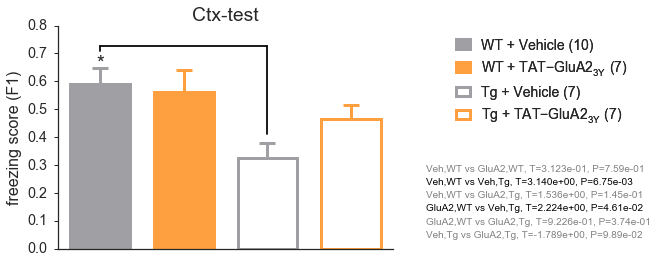
\includegraphics[width=\textwidth]{nb.png}
        \caption{\label{f.ad.nb}}
    \end{subfigure}
    \begin{subfigure}[h]{\textwidth}
        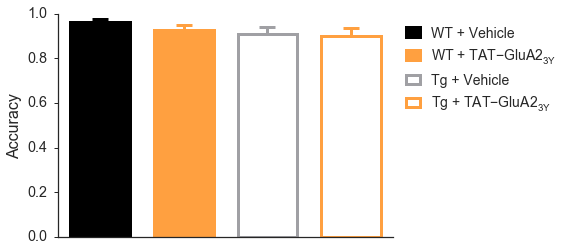
\includegraphics[width=\textwidth]{svm.png}
        \caption{\label{f.ad.svm}}
    \end{subfigure}
    \caption{Performance of \subref{f.ad.nb} \gls{nbc} and \subref{f.ad.svm} \gls{gsvm} in predicting freezing from cell activity. Results are measured  using the F1 score. Both classifiers showed significant lower performance in \gls{tg} group, further supports the hypothesis that \gls{tg} mice have deficits in encoding freezing during the context memory test. Interestingly, since \gls{nbc} assumes the cells are independent and \gls{gsvm} is more general, the performance difference between the two suggest a portion of freezing information is encoded in the network level. \label{f.ad.classifier}}
\end{figure}


\subsection{Freezing encoding precedes freezing behaviour}


\begin{figure}[h]
    \centering
    \begin{minipage}[b]{0.45\linewidth}
        
\begin{tikzpicture}
    \node[obs] (acc) {acc};
    \node[latent, left= of acc] (sig) {$\sigma$};
    \node[det, above= of acc] (mu) {$\mu$};     
    \node[obs, above=of mu] (t) {$t$};
    \node[latent, left=of t] (mu0) {$\mu_0$};
    \node[latent, right= of mu] (s) {$s$};
    \node[latent, left=of mu] (tau) {$\tau$};
    \node[latent, right=of t] (a) {$a$};

    \edge {tau,s,t,mu0,a} {mu};
    \edge {mu, sig} {acc};
   
    \plate{tplate} {(t) (mu) (acc)} {$\forall t \in [T_{min}, 0)$};
\end{tikzpicture}

    \end{minipage}
    \begin{minipage}[b]{0.45\linewidth}
        \begin{align*}
            \mu_0 &\sim \operatorname{Gaussian}(0, 1000) \\
            a &\sim \operatorname{Gaussian}(0, 1000) \\
            a &> 0 \\
            \tau &\sim \operatorname{DiscreteUniform}(T_{min}, 0) \\
            s &\sim \operatorname{Bernoulli}(0.5) \\
            acc &\sim \operatorname{Gaussian}(\mu, \sigma) \\
            \mu &=
                \begin{cases}
                    \mu_0 & \text{if }s=0\text{ or }t>\tau \\
                    \mu_0 - a(t-\tau) & \text{otherwise}
                \end{cases}
        \end{align*}
    \end{minipage}
    \caption{Bayes model for change point detection. The accuracy is modelled as a Gaussian distribution with mean as a function of time and constant variance. In the null hypothesis, the mean is constant and estimated from the data. In the alternative hypothesis, the mean is modelled as constant up to the change point, then as a linear function of time with a negative slope. A Bernoulli variable $selector$ is estimated to choose from each of the hypothesis. All variables have non-informative priors \label{f.ad.bayesmodel}}
\end{figure}

We next examined whether freezing encoding in the network precedes behaviour onset. \todo{relate to literature} We plotted average prediction accuracy for the classifiers at the time mice behaviour transitions into freezing. We hypothesized that if the neural signiture for freezing behaviour in the network precedes, the classifiers will predict freezing earlier than the behavioural onset, which will result in a reduction prediction accuracy before behavioural onset.

We used Bayes modelling (Figure \ref{f.ad.bayesmodel}) to detect whether the prediction accuracy changes before behaviour change, and compared change points between groups. The result is summarized in Figure~\ref{f.ad.into_f}. We have found very strong evidence for a change point in \gls{nbc} performance in every group (all Bayes factors BF\tsb{10} > \num{5e4}). The change point appears $3.4_{-0.1}^{+0.1}$\SI{}{\s} in WT-Veh, $2.8_{-0.1}^{+0.1}$\SI{}{\second} in WT-\glu, $2.8_{-0.3}^{+0.2}$\SI{}{\second} in Tg-Veh, and $2.6_{-0.1}^{+0.1}$\SI{}{\second} in Tg-\glu before freezing onset (uncertainties are \SI{95}{\percent} credible intervals). Pairwise comparisons show very strong evidence that the change point in WT-Veh occurs earlier than the other three groups, while the other three groups occur at the same time (WT-Veh vs WT-\glu, BF\tsb{10} > \num{250}; WT-Veh vs Tg-Veh, BF\tsb{10} = \num{7.5}; WT-Veh vs Tg-\glu, BF\tsb{10} > \num{250}; all other comparisons BF\tsb{10} < \num{0.2}). Since \gls{nbc} regards each cell independently, this result suggest that the freezing signal in individual cells occurs earlier than the onset of freezing behaviour.

On the other hand,  we have found very strong evidence for a change point in \gls{gsvm} performance in WT-Veh (BF\tsb{10} > \num{5e4}), WT-\glu (BF\tsb{10} > \num{5e4}) and Tg-\glu (BF\tsb{10} > \num{5e4}), and also strong evidence that a change point does not present in Tg-Veh (BF\tsb{10} < \num{0.02}). The change points are estimated to be $0.6_{-0.1}^{+0.0}$\SI{}{\s} in WT-Veh, $2.6_{-0.3}^{+0.2}$\SI{}{\second} in WT-\glu, and $0.3_{-0.2}^{+0.1}$\SI{}{\s} in Tg-\glu, before the freezing onset. Pairwise comparisons show very strong evidence of a earlier change point in WT-\glu than the other groups (WT-\glu vs WT-Veh, BF\tsb{10} > \num{250}; WT-\glu vs Tg-\glu, BF\tsb{10} > \num{250}). There is minimal evidence that the change point in WT-Veh is earlier than Tg-\glu (BF\tsb{10} = \num{2.5}). These results suggest that the network neural signature for freezing occur earlier than freezing behaviour in \gls{wt} groups, however not detected in the \gls{tg} group. \tglu treatment of the \gls{tg} mice is able to partially rescues this effect. In addition, the network freezing signal occur earlier in WT-\glu than the other groups. These results suggest that the \tglu treatment helps strengthen the network signal, both in \gls{wt} and \gls{tg} mice. \todo{explain} 


\begin{figure}[h]
    \begin{subfigure}[h]{\textwidth}
        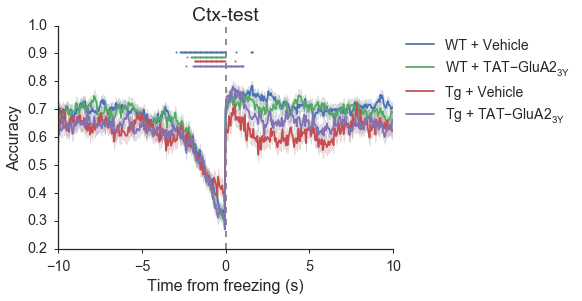
\includegraphics[width=\textwidth]{nb_into_freezing.png}
        \caption{\label{f.ad.nb_into_f}}
    \end{subfigure}
    \begin{subfigure}[h]{\textwidth}
        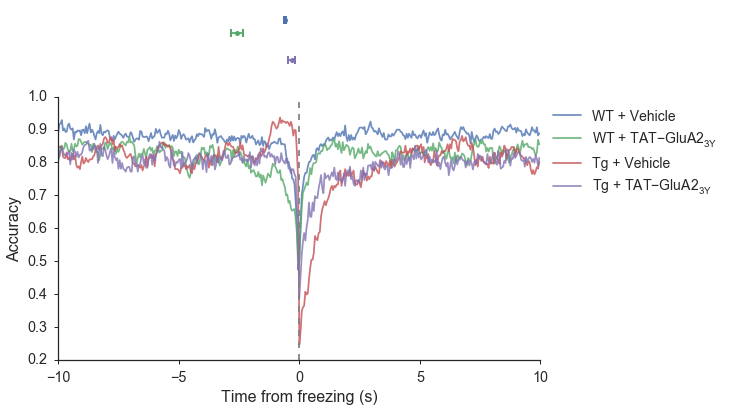
\includegraphics[width=\textwidth]{svm_into_freezing.png}
        \caption{\label{f.ad.svm_into_f}}
    \end{subfigure}
    \caption{Average accuracy of classifiers at the beginning of freezing behaviour in mice during the context memeory test. For \gls{wt} and \gls{tg}-\glu groups, both \gls{nbc} and \gls{gsvm} shows significantly decreased performance just before the mice show freezing behaviour. This suggests that \gls{ca1} neural activity drives freezing behaviour. The error bars on the top shows \SI{95}{\percent} credible interval of the change point, if the alternative hypothesis is favoured. \label{f.ad.into_f}}
\end{figure}


\subsection{\Gls{tg} mice have deficits recall freezing memory}

\todo{short-term memory}

Given that \gls{tg} mice have significant neuronal signal before freezing, and they are able to initiate freezing as often as \gls{wt} mice, we hypothesized that they have deficits in memory recall rather than memory encoding. \todo{relate to lit., e.g. tonegawa paper, and reinstatement}

To test this hypothesis, we trained \gls{wt} and \gls{tg} mice treatment-free, and \SI{3}{\day} later, treated the mouse with \tglu or saline vehicle when they are shortly exposed to the training context as a reminder. The memory test occurred \SI{24}{\hour} later. The result is summarized in Figure~\ref{f.ad.reminder1}. We found a significant interaction between genotype and treatment (\todo{stats}). \textit{Post hoc} tests shows Tg-Veh has a significant memory deficit (\todo{stats}), however this effect is fully rescued by \tglu treatment (\todo{stats}). This result suggests that \gls{tg} mice have intact memory encoding and deficits in memory recall. The recall deficit can be rescued with \tglu treatment if the mouse is exposed to a reminder.

\begin{figure}[h]
    \begin{subfigure}[h]{\textwidth}
        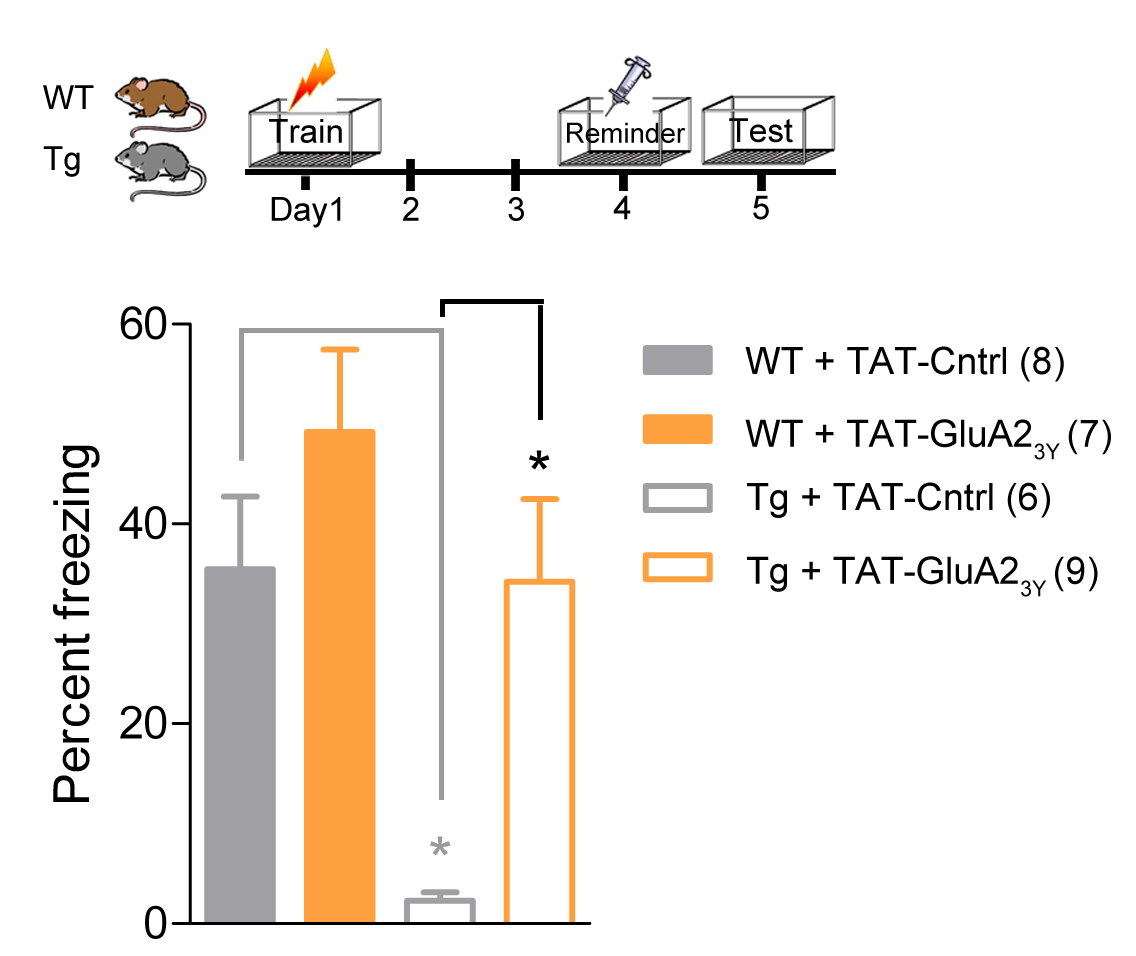
\includegraphics[width=\textwidth]{reminder1.png}
        \caption{\label{f.ad.actf}}
    \end{subfigure}
    \caption{\gls{tg} mice have deficits in memory recall but not memory encoding. \gls{wt} and \gls{tg} mice were contextual fear conditioned, given a reminder \SI{3}{\day} later with treatment and tested on the following day. \gls{tg} mice showed significantly less freezing, however this effect is rescued by \tglu treatment. \label{f.ad.reminder1}}
\end{figure}

We then investigated whether the effect of the \tglu is memory specific. In a separate cohort of mice, we use a similar protocol as Figure~\ref{f.ad.reminder1}, except the mice received \tglu in their home-cage instead of the reminder (Figure~\ref{f.ad.reminder2}). In this case, the \tglu treatment does not have any effect on memory recall. There is a significant main effect of genotype (\todo{stats}), and the genotype $times$ treatment interaction is not significant (\todo{stats}; Figure~\ref{f.ad.reminder2}). Together, these two pieces of results suggest that \gls{tg} mice have normal memory encoding but unable to recall, and \tglu can rescues the recall deficit during reinstatement. 


\begin{figure}[h]
    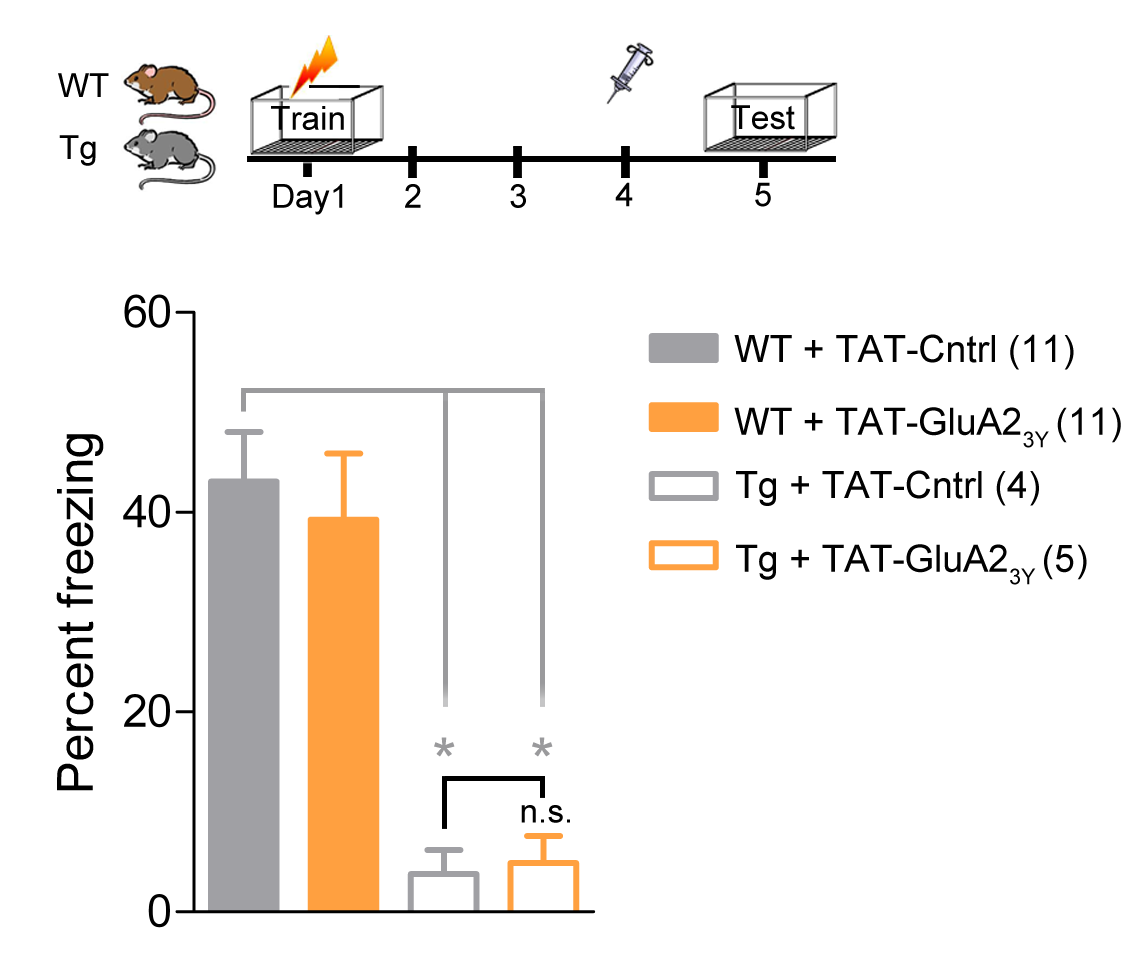
\includegraphics[width=\textwidth]{reminder2.png}
    \caption{\tglu does not rescue memory recall without reminder. \gls{wt} and \gls{tg} mice were contextual fear conditioned, given treatment in home cage and tested on the following day. \tglu treatment without reminder is unable to rescue recall deficit in \gls{tg} mice. \label{f.ad.reminder2}}
\end{figure}

\section{Discussion}


In the current project, we took advantage of our home-made miniature microscope to record \gls{ca1} cells in WT and a mouse model of early \gls{ad}, TgCRND8 mice, during contextual fear conditioning. We have found a significant memory deficit in TgCRND8 mice. Correlated with the memory deficit, we have also discovered that the TgCRND8 mice have hyperactive \gls{ca1} neurons. Compared to the WT mice, the \gls{ca1} neurons in the TgCRND8 mice contain reduced information content about the mice's behavioural state of memory recall. The reduction of information content is independent to spatial encoding and the strength of memory (as measured by proportion of time the mice spent freezing), suggesting that this reduction of information content is related to a specific memory deficit in the TgCRDN8 mice.

To investigate the ensemble encoding of the fear memory, we trained machine learning classifiers to predict, at each time point, the behavioural state of memory recall using the calcium activity in the neurons. To differentiate the cellular and network activity, we used \gls{nbc} and \gls{gsvm} and compared results obtained from both classifiers. \Gls{nbc} is only able to detect signals when each neuron is treated as independent from others, while \gls{gsvm}, being a general classifier, is able to utilize all available information, including those both in the individual cell level, and also information stored in the higher order relationship between the activity of cells. 

The first finding from the prediction accuracy of the classifiers is although deficit at encoding memory recall in individual cells, as measured by mutual information content, with multiple neurons, the classfiers are able to decode at similar accuracy level between TgCRND8 and WT mice. This suggests that although the physiology of individual cells are significant impacted by the TgCRND8 phenotype, neurons as a network can largely compensate information encoding. This is also supported by the finding that the \gls{gsvm} perform significant better than the \gls{nbc}, suggesting that a significant portion of the information for memory recall is stored in the coorperative activity of neurons. 

To investigate how the degradation of the cell firing in \gls{ca1} neurons in the TgCRND8 mice contributes to the memory deficit, we then investigated whether the important circuitry function of hippocampus, pattern completion, which is necessary for memory recall, is affected in the TgCRND8 mice. While the Marr Model and empirical evidence more recently \citep{rolls13, neunuebel14} suggest that \gls{ca3} the the major site in hippocampus where pattern completion occur, however given that the input--output difference in \gls{ca1} is relative linear \citep{neunuebel14, knierim16}, the pattern completion process should also be reflected in \gls{ca1}, and can be detected in our recording. 

To observe the pattern completion process, we have aligned the classifier performances to the time when the mice begin to freeze. In \gls{nbc}, we observed a decrease in prediction accuracy just before the mice start to freeze. The decrease of prediction accuracy is a result of the classifier misclassifying non-freezing to freezing. This shows that the classifier starts to predict the mice to freezing just before the behavioural change. There is no between-group difference in the \gls{nbc} prediction accuracy, however while the WT group shows similar prediction precedance in \gls{gsvm}, this precedance is missing for \gls{gsvm} prediction in the TgCRND8 mice. 

Since the classifiers are trained to recognize specific neural activity pattern for the fear memory, the precedance of classifier prediction to behaviour suggest that the \gls{ca1} activity pattern for the fear memory leads behaviour. The gradual rise of the classifier's prediction before freezing also suggest that pattern of fear memory arise dynamically: the fear memory pattern starts as a partial pattern which can only barely detected by the classifier, and this gradually develop into a full pattern which biases the prediction of the classifier. 

The difference of temporal dynamics of the ``pattern completion'' process has also hinted the underlying dynamic mechanism of the process. Since the \gls{nbc} is only able to detect activity pattern at individual cell level, the rise of fear prediction in \gls{nbc} suggest that individual cells start show a the firing pattern of the fear memory. On the other hand, the \gls{gsvm} detects network pattern, which is composed of synchronized activity of indiviual cells. We have found the \gls{nbc} prediction precedes the \gls{gsvm} prediction, suggesting that the fear memory pattern in the \gls{ca1} start as an incomplete pattern composed of unsynchronized individual cell activity, and the cellular pattern completes, it leads to synchronized network activity, and are detected by the \gls{gsvm} later on. 

The difference of the TgCRND8 mice and WT mice can also be interpreted in this framework. The TgCRND8 mice display similar dynamics in \gls{nbc}, suggesting that the cellular signals are not affected. However, the missing of a dynamic pattern completion process in the \gls{gsvm} suggesting that which the individual cells are able to response to the initiation of a fear memory, the cells are unable to coordinate to form a network pattern. 

The inability of the TgCRND8 mice to coordinate and form a network pattern is better shown in \todo{ref figure}, where we investigated the relative distance of network state to the \gls{gsvm} classifier boundary. Given the high accuracy of the \gls{gsvm} prediction, the \gls{gsvm} classifier boundary can approximate the actual behaviour state transition boundary. We found the TgCRND8 mice approaches the fear memory state later, and also shallower than the \gls{wt} mice, this further confirms a deficit in the pattern completion process. 

Interestingly, treating the TgCRND8 mice with \tglu during memory formation is able to rescue all of the cellular, network and behavioural deficit we have found. TgCRND8 mice with \tglu treatment is able to show normal expression of fear memory. The \tglu treatment is able to decrease the cell excitabliity in TgCRND8 mice, and allow the activity of the cells to be as informative as \gls{wt} mice about the behavioural state of the memory recall. Moreover, the \tglu treatment is also able to rescue the pattern completion deficit. 

Some of the effect of the \tglu treatment is also reflected on \gls{wt} mice. While the \tglu treatment have no effect on the overall cell activity in \gls{wt} mice, when we control movement of the mice and only compare cell activity during freezing, we found \tglu decreases cell activity even in \gls{wt} mice. Moreover, \tglu treatment in \gls{wt} mice also leads the classifier to predict freezing earlier than vehicle-treated \gls{wt} mice, which is evidence for an enhancement of the pattern completion process. 

The memory deficit of the TgCRND8 mice can be a deficit of memory formation, or a deficit of memory recall. To test this hypothesis, we trained \gls{wt} and TgCRND8 mice, and only treated the mice with vehicle or \tglu on the next day, when the mice is briefly exposed to a reminder. The memory is tested on the following day. We found that while TgCRND8 mice show a memory deficit, \tglu treatment during reminder is able to completely rescue the memory deficit. However interestingly, the presence of the reminder is crucial for the rescuing effect of \tglu, as \tglu treatment when the mice is in their home cage does not have an effect on memory recall. 

These two pieces of results suggest that first, TgCRND8 mice is still able to form a contextual fear memory. This is because if otherwise the memory is not formed during training, \tglu treatment with reminder should not have any rescuing effect, as the memory would not be present at that time point. However, the fact that the rescuing effect of \tglu requires the presence of the reminder suggest that the effect of \tglu is not universal, and the effect is specific to the current active memory trace. 

In conclusion, we have found that the TgCRND8 mice is able to learn a contextual fear memory, however unable to recall it. This deficit is accompanied by, a hyperactive \gls{ca1} and decreased information content in the \gls{ca1} cells. While the behaviour information can still be decoded using activity of a neural population, cells in TgCRND8 is unable to pattern complete a conextual fear memory. This deficit may explain the recall deficit in these mice. Moreover, all the deficit can be rescued by \tglu treatment during training. Given the effect of the \tglu on synaptic strengthening, the current study is able to link synaptic functions to neural circuits in \gls{ca1}, and ultimately behaviour. While the mechanism of how effect of the synaptic function creates the changes of \gls{ca1} neural circuit function is still unclear, this study have created a potential link of circuit function from molecular and behaviour, as well as demonstrated the importance of understanding circuit function in the study of the \gls{ad}, and also suggested potential novel treatment target of \gls{ad} at a neural circuitry level. 

